%\documentclass[sigconf, anonymous, review]{acmart}
\documentclass[sigconf, anonymous]{acmart}


\usepackage{colortbl}
\usepackage{tikz}
%\usepackage{arydshln}
\usepackage{multirow}
\usepackage{amssymb}
\setcounter{tocdepth}{3}
\usepackage{graphicx}
\usepackage{makecell}
\usepackage{enumitem}
%\usepackage{todonotes}
\usepackage{multirow}   % Allows table elements to span several rows.
\usepackage{booktabs}   % Improves the typesettings of tables.
\usepackage{hyperref}  % Enables cross linking in the electronic document version. This package has to be included second to last.

\usepackage{booktabs,arydshln}
%\usepackage[usenames,dvipsnames,table]{xcolor}


%\newcommand{\mytodo}[1]{\textcolor{red}{#1}}

\makeatletter
\def\adl@drawiv#1#2#3{%
        \hskip.5\tabcolsep
        \xleaders#3{#2.5\@tempdimb #1{1}#2.5\@tempdimb}%
                #2\z@ plus1fil minus1fil\relax
        \hskip.5\tabcolsep}
\newcommand{\cdashlinelr}[1]{%
  \noalign{\vskip\aboverulesep
           \global\let\@dashdrawstore\adl@draw
           \global\let\adl@draw\adl@drawiv}
  \cdashline{#1}
  \noalign{\global\let\adl@draw\@dashdrawstore
           \vskip\belowrulesep}}
\makeatother


% Copyright
%\setcopyright{none}
%\setcopyright{acmcopyright}
%\setcopyright{acmlicensed}
\setcopyright{rightsretained}
%\setcopyright{usgov}
%\setcopyright{usgovmixed}
%\setcopyright{cagov}
%\setcopyright{cagovmixed}


% DOI
%\acmDOI{10.475/123_4}

% ISBN
%\acmISBN{123-4567-24-567/08/06}

%Conference
\acmConference[SIGIR'18]{The 41st International ACM SIGIR Conference on Research and Development in Information Retrieval}{June 2018}{Ann Arbor, Michigan, U.S.A.} 
%\acmYear{1997}
%\copyrightyear{2016}

%\acmArticle{4}
%\acmPrice{15.00}

% These commands are optional
%\acmBooktitle{Transactions of the ACM Woodstock conference}
%\editor{Jennifer B. Sartor}
%\editor{Theo D'Hondt}
%\editor{Wolfgang De Meuter}

\newcommand{\mytodo}[1]{\textcolor{red}{#1}}
\newcommand{\todo}[1]{\textcolor{red}{#1}}

\hyphenation{Wiki-pedia}

\begin{document}

%\title{A new Framework for Multi-Dimensional Evaluation Metrics in Search Engines}

\title{A new Framework for\\ Multidimensional Evaluation of Search Engines}

%\titlenote{Produces the permission block, and copyright information}
%\subtitle{Extended Abstract}
%\subtitlenote{The full version of the author's guide is available as \texttt{acmart.pdf} document}


% The default list of authors is too long for headers.
\renewcommand{\shortauthors}{Author et al.}

\begin{abstract}
In this paper, we investigated methods to estimate the understandability of health Web pages and used these to improve the retrieval of information for people seeking health advice on the Web.  Understandability plays a key role in ensuring that people accessing health information are capable of gaining insights that can assist them with their health concerns and choices. The access to unclear or misleading information has been shown to negatively impact on the health decisions of the general public. 

Our investigation considered methods to automatically estimate the understandability of health information in Web pages, and it provided a thorough evaluation of these methods using human assessments as well as an analysis of pre-processing factors affecting understandability estimations, and associated pitfalls. Furthermore, lessons learnt for estimating Web page understandability were applied to the construction of retrieval methods with specific attention to retrieving information understandable by the general public.

We found that machine learning techniques were more suitable to estimate health Web page understandability than traditional readability formulas, which are often used as guidelines and benchmarking by health information providers on the Web. Learning to rank effectively exploited these estimates to provide the general public with more understandable search results. These results are important for specialised search services tailored to support the general public in seeking health advice on the Web.


\end{abstract}




%
% The code below should be generated by the tool at
% http://dl.acm.org/ccs.cfm
% Please copy and paste the code instead of the example below. 
%
%\begin{CCSXML}
%<ccs2012>
% <concept>
%  <concept_id>10010520.10010553.10010562</concept_id>
%  <concept_desc>Computer systems organization~Embedded systems</concept_desc>
%  <concept_significance>500</concept_significance>
% </concept>
% <concept>
% <concept_id>10010520.10010575.10010755</concept_id>
% <concept_desc>Computer systems organization~Redundancy</concept_desc>
% <concept_significance>300</concept_significance>
%</concept>
%<concept>
% <concept_id>10010520.10010553.10010554</concept_id>
% <concept_desc>Computer systems organization~Robotics</concept_desc>
% <concept_significance>100</concept_significance>
%</concept>
%<concept>
% <concept_id>10003033.10003083.10003095</concept_id>
% <concept_desc>Networks~Network reliability</concept_desc>
% <concept_significance>100</concept_significance>
%</concept>
%</ccs2012>  
%\end{CCSXML}

%\ccsdesc[500]{Computer systems organization~Embedded systems}
%\ccsdesc[300]{Computer systems organization~Redundancy}
%\ccsdesc{Computer systems organization~Robotics}
%\ccsdesc[100]{Networks~Network reliability}


%\keywords{ACM proceedings, \LaTeX, text tagging}

\maketitle

\section{Evaluation Metrics of Understandability in Search Engines}
\label{chp:evaluation_metrics}

One of the first notions of relevance was straightforward: a document is relevant to a query if the topic of the information retrieved matches the topic of the request.
This was called \textit{topical relevance} by Eisenberg and Schamber~\cite{eisenberg88} and measured whether a document was ``on the topic'' or ``on the subject''.
Due to its simplicity and clear definition~\cite{borlund03}, this notion was adopted by most of the modern evaluation tasks, such as TREC\footnote{\url{http://trec.nist.gov}}, CLEF\footnote{\url{http://www.clef-initiative.eu/}} and NTCIR\footnote{\url{http://http://research.nii.ac.jp/ntcir/index-en.html}}, which heavily rely on evaluation metrics that exclusively measure the topical relevance of documents~\cite{voorhees05}.
Recently extensions were made based on notions of novelty and diversity (e.g.,~\cite{clarke09}), but these new metrics still mainly consider relevance with respect to document topicality.

However, document relevance cannot be attributed to just one factor such as topicality, instead it is multidimensional and situational~\cite{borlund03}.
Early research~\cite{saracevic75,swanson86,harter92}, reviewed by Borlund divided relevance into two classes: (1) objective or system-based relevance and (2) subjective or human based relevance~\cite{borlund03}. 
This first class of relevance exclusively refers to the document ``aboutness'' aforementioned and it is context-free, while the second one refers to the subjective factors in both user and documents and it is context dependent.
A large body of subsequent research was dedicated to identifying the subjective aspects of relevance.
Park, for example, identified individual's subject knowledge, professional training, and educational background as a user-based influential factor, while scarcity, availability, timeliness, and scope as document-based factors~\cite{park93}.
Schamber published a compiling and non-exhaustive list of 80 relevance criteria suggested in the literature~\cite{schamber94}.
%
In the consumer health search domain, William Hersh highlighted two important factors to be considered by modern search engines~\cite{hersh08}: understandability and information trustworthiness. 
This paper focus on the community efforts to integrate these two dimensions in the evaluation of consumer health search systems.
%This thesis focus on the first one.

Early efforts to integrate understandability into information retrieval evaluation was made by Zuccon and Koopman~\cite{zuccon14} and enhanced later by Zuccon~\cite{zuccon16}.
Metrics such as $uRBP$ and $uRBPgr$, built upon the Rank Biased Precision metric (RBP)~\cite{moffat08}, were widely used in recent evaluation campaigns in the context of CLEF eHealth to combine understandability of documents with topical relevance.
$uRBP$, short for understandability-biased RBP and its graded version, $uRBPgr$, merge the relevance and understandability scores of a document into a unique score following the gain-discount framework by Carterette~\cite{carterette11}.

While Zuccon's framework can be successfully used to compare results across systems, as intended by evaluation campaigns such as CLEF eHealth, it is not trivial to identify how the retrieval performance of different dimensions affect the final score outputted by this framework.
We shall see in this paper that the early combination of scores make it difficult to interpret whether improvements (deterioration) are due to more (less) understandable or more (less) topical documents being retrieved.

What We propose is an alternative metric $H$ which uses a harmonic mean function to combine scores earlier calculated for each dimension.
In order to fairly compare our framework with Zuccon's, we also modify the RBP metric in our framework, resulting in the $H_{RBP}$ metric.

We shall review Zuccon's framework in Section~\ref{sec:understandability_metrics}. 
Our proposed alternative framework is presented in Section~\ref{sec:extension}.
We compare both frameworks through simulations in Section~\ref{sec:simulations}.
Finally, a summary is done in Section~\ref{sec:eval_summary}.

%%%%%%%%%%%%%%%%%%%%%%%%%%%%%%%%%%%%%%%%%%%%%%%%%%%%%%%%%%%%%%%%%%%%%%%%%%%%%%%%%%%%%%%%%%%%%%%%%%%%%%%%%%%%%%%%%%%%%%%%%%%%%%%%
%%%%%%%%%%%%%%%%%%%%%%%%%%%%%%%%%%%%%%%%%%%%%%%%%%%%%%%%%%%%%%%%%%%%%%%%%%%%%%%%%%%%%%%%%%%%%%%%%%%%%%%%%%%%%%%%%%%%%%%%%%%%%%%%
%%%%%%%%%%%%%%%%%%%%%%%%%%%%%%%%%%%%%%%%%%%%%%%%%%%%%%%%%%%%%%%%%%%%%%%%%%%%%%%%%%%%%%%%%%%%%%%%%%%%%%%%%%%%%%%%%%%%%%%%%%%%%%%%
%%%%%%%%%%%%%%%%%%%%%%%%%%%%%%%%%%%%%%%%%%%%%%%%%%%%%%%%%%%%%%%%%%%%%%%%%%%%%%%%%%%%%%%%%%%%%%%%%%%%%%%%%%%%%%%%%%%%%%%%%%%%%%%%



\section{Incorporating Understandability into Evaluation Metrics}
\label{sec:understandability_metrics}
The understandability-biased IR evaluation framework (UBIRE)~\cite{zuccon14,zuccon16} is based on the gain-discount framework~\cite{carterette11} which models an evaluation measure $\mathcal{M}$ as:

\vspace{-4pt}
\begin{equation*}
\mathcal{M} = \frac{1}{\mathcal{N}} \sum_{k=1}^{K} \mathtt{d}(k) \mathtt{g}(d@k)
\end{equation*}
%
where $\mathtt{g}(d@k)$ and $\mathtt{d}(k)$ are respectively the \textit{gain function} computed for the (relevance of the) document at rank $k$ (i.e. $d@k$) and the \textit{discount function} computed for the rank $k$.
$K$ is the depth of assessment at which measure $\mathcal{M}$ is evaluated, and $1/\mathcal{N}$ is an optional normalization factor, which serves to bound the value of the sum into the range [0,1] (details in~\cite{carterette11}).

The gain-discount framework encompasses measures such as the normalized Discounted Cumulative Gain (nDCG)~\cite{jarvelin02} with $\mathtt{g}(d@k) = 2^{P(R|d@k)} - 1$ and $\mathtt{d}(k) = 1/(log_2(1 + k))$; the expected reciprocal rank (ERR)~\cite{chapelle09} with $\mathtt{g}(d@K) =  (2^{P (R|d@k)} - 1)/2^{max(P (R|d))}$ and $\mathtt{d}(k) = 1/k$; and the Rank Biased Precision (RBP) with $\mathtt{g}(d@k)$ equal to 1 if $d@k$ is relevant and 0 otherwise and $\mathtt{d}(k) = \rho^{k-1}$ (with $\rho$ representing the user persistence).

The gain provided by a document at rank $k$ can be expressed as a function of its probability of relevance. Without loss of generality, $\mathtt{g}(d@k) = f(P(R|d@k))$, where $P(R|d@k)$ is the probability of relevance given the document at $k$. 
When only topical relevance is modelled, then $P(R|d@k) = P(T|d@k)$, i.e., the probability that the document at $k$ is topically relevant. 
For binary relevance, this probability is 1 for relevant documents and 0 for non-relevant documents. For non-binary relevance, this probability can be distributed according to the number of relevance levels.

UBIRE extends this framework to consider cases where relevance is modelled beyond topicality so as to explicitly model other dimensions, such as understandability.
This is done by modelling the probability of relevance $P(R|d@k)$ as the joint distribution over all considered dimensions, $P(\delta_1, \cdots, \delta_n|d@k)$, where each $\delta_i \in \mathcal{D}$ represents a dimension of relevance, e.g., topicality, understandability. The computation is simplified by assuming that dimensions are compositional events and their probabilities independent (see~\cite{zuccon16} for more details). The gain function with respect to different dimensions of relevance can then be expressed as:
%
%\begin{eqnarray}
%    g(d@k) &=& f(P(R|d@k)) \\
%    &=& f\big(P(D_1, \cdots, D_n|d@k)\big) \\
%    &=& f\Big(\prod_{i=1}^n P(D_i|d@k)\Big) 
%\end{eqnarray}
%
% Alternative:
\begin{eqnarray*}
    \mathtt{g}(d@k) &=& f(P(R|d@k)) \\
    &=& f\big(P(\delta_1, \cdots, \delta_n|d@k)\big) = f\Big(\prod_{i=1}^n P(\delta_i|d@k)\Big) 
\end{eqnarray*}


Evaluation metrics developed within this framework differ by means of the instantiations of $f\big(P(\delta_1, \cdots, \delta_n|d@k)\big)$, other than by which dimensions are modelled. Zuccon provided an instantiation that considers both topicality and understandability~\cite{zuccon16}:
%
\begin{equation*}
\mathtt{g}(d@k) = f(P(R|d@k)) = f\big(P(T|d@k) \cdot P(U|d@k)\big)
\end{equation*}
%
%with $P(R|d@k)$ as the joint $P(T,U|d@k)$ that is in turn computed as the product $P(T|d@k) \cdot P(U|d@k)$ following the assumptions discussed above.

Specific implementations of the UBIRE framework that have been developed in previous work considered the basic gain and discount functions from RBP~\cite{moffat08}; an instantiation with understandability~\cite{zuccon14,zuccon16} has been later extended by jointly considering also trustworthiness~\cite{clefIR17}. For ease of explanation, we consider the formulation with topicality and understandability; similar considerations apply when also trustworthiness is modelled (as well as other dimensions, as a matter of fact). In this case, the understandability-biased RBP, $uRBP$, is defined as: 
%
\begin{eqnarray*}
    uRBP(\rho) &=& (1-\rho) \sum_{k=1}^{K} \rho^{k-1} P(T|d@k) \cdot P(U|d@k)\\ 
&=& (1-\rho) \sum_{k=1}^{K} \rho^{k-1} \mathtt{g}_{RBP}(d@k) \cdot \mathtt{g}_{U}(d@k)
\label{eq:RBP}
\end{eqnarray*}


%%%Specifically, Zuccon~\cite{zuccon16} provided an instantiation of this multidimensional evaluation approach on top of RBP~\cite{moffat08}, a well understood metric of retrieval effectiveness which also fits within the gain-discount framework. 
%%In the context of RBP, the gain function $r(d@k)$ is 1 if $d@k$ is relevant and 0 otherwise, the discount function is measured by a geometric function of the rank, i.e., $d(k) = \rho^{k-1}$ (with $\rho$ representing the user persistence), and $1-\rho$ acts as a normalization component. Putting all together, RBP is expressed by the following formula:
%%%)
%%\begin{equation}
%%    RBP(\rho) = (1-\rho) \sum_{k=1}^{K} \rho^{k-1} r(d@k)
%%\label{eq:RBP}
%%\end{equation}
%%%
%%Note that $r(d@k)$ is an initialization of $f(P(T|d@k))$, where $f(.)$ is the identity function and $r(d@k)$ estimates $P(T|d@k)$. 

%Extending RBP to cope with multidimensional relevance, Zuccon and Koopman~\cite{zuccon14} define the understandability-biased RBP, $uRBP$, as: 
%%
%\begin{eqnarray}
%    uRBP(\rho) &=& (1-\rho) \sum_{k=1}^{K} \rho^{k-1} P(T|d@k) \cdot P(U|d@k)\\ 
%&=& (1-\rho) \sum_{k=1}^{K} \rho^{k-1} r(d@k) \cdot u(d@k)
%\label{eq:RBP}
%\end{eqnarray}
%
In the $uRBP$, the function $\mathtt{g}_{RBP}(d@k)$ is the same as the gain in RBP and transforms relevance values into the corresponding gains and, likewise, $\mathtt{g}_{U}(d@k)$ transforms understandability values into the corresponding gains. 
If $\mathtt{g}_{U}(d@k)=1$ for every document, then only topical relevance affects retrieval evaluation, i.e. every document is considered as having equal understandability (and its highest value) and we obtain the original RBP. Two instantiations of the gain function $\mathtt{g}_{U}(d@k)$ have been explored in previous work: one binary (\textit{uRBP}) and the other graded (\textit{uRBPgr}). In the binary version $\mathtt{g}_{U}(d@k) = 1$ if $P(U|d@k) \geq th_U$, where $th_U$ is a threshold on the assessments of understandability (every assessment that is greater than or equal to $th_U$ would generate a gain of 1), and $\mathtt{g}_{U}(d@k)=0$ otherwise. In the graded version, understandability assessments are transformed into estimations of the probability function $P(U|d@k)$.
% In case we need space, I would remove the following sentences:
%\mytodo{Remove the following sentences?}
%For example, assessments collected on a Likert scale of 5 levels have been converted into estimations ranging from 0.0 to 1.0 with steps of 0.25 (0.0, 0.25, 0.50, 0.75 and 1.0)\todo{~\cite{}}.
%Assessments collected on a scale $[0,100]$ have been directly used as estimations of $P(U|d@k)$ or modified using a smoothing function\todo{~\cite{}}.


%Next we define how $r(d@k)$, $u(d@k)$ and $t(d@k)$ are computed.
%While $r(d@k)$ is the same function as in the original version of RBP, i.e. the binary function returning 1 if the document is relevant and 0 otherwise, $u(d@k)$ might have two different instantiations: one binary and the other graded. The binary version simply assumes $u(d@k)$ as a binary function that returns 1 if $P(U|d@k) \geq th_U$ and 0 otherwise, where $th_U$ is a threshold on the assessments of understandability. 
%For the graded version, we rely on understandability assessment collected on a scale from 0\% to 100\% (0\% being the lowest level of understandability), convert these to probabilities and use the assessments as estimations of $P(U|d@k)$. These estimations are then directly plugged into the measure. In order to distinguish binary from graded measures, Zuccon adds the suffix \textit{gr} to the graded version of the measures~\cite{zuccon16}.
%For the graded version, we rely on the possibility to transform the understandability assessment collected into estimations of $P(U|d@k)$.
%For example, assessments collected in a Likert scale of 5 levels can be easily converted into estimations ranging from 0.0 to 1.0 with steps of 0.25 (0.0, 0.25, 0.50, 0.75 and 1.0).
%Assessments collected in a scale from 0 to 100 (e.g., 0 being the lowest level of understandability), could be directly used as estimations of $P(U|d@k)$ or modified by a smoother function.
%These estimations are then plugged into the metric. In order to distinguish binary from graded metrics, the suffix \textit{gr} was added to the graded version of the metrics~\cite{zuccon16}.

%\todo{maybe move this paragraph to the actual experimentation part}
%The settings used in CLEF eHealth 2015 was to attribute the value of 0.0 to $P(U|d@k)$ if a document was assessed as hard to understand, 0.4 if it was assessed as somewhat hard to understand, 0.8 for a somewhat easy-to-understand document and, finally, 1.0 if the document was assessed as easy to understand. In CLEF eHealth 2016, assessments were made in a 0-100 scale, with 0 being the easiest to read, thus $P(U|d@k)$ was assigned as (100 - understandability\_label)/100.
%Also, the RBP's $\rho$ parameter was set to 0.80~\cite{clef15,clef16}. We shall use the same definitions in \mytodo{Chapter XXX}.

% The goal of CLEF eHealth 2015 and 2016 was to retrieve documents as easy as possible, but that might not always be the case. A user with larger health domain knowledge might accept -- or even want -- a harder document to read.

%The method we use to define the graded version of the multidimensional measures differs from that used in~\cite{zuccon16}, where instead categorical assessments of understandability were mapped to (arbitrary) gain values. We believe that our use of a continues scale to measure these dimensions and assign the corresponding gains is more appropriate to the task, provides a finer grained evaluation of the systems, and also better aligns with the original assessments captured in the CLEF eHealth 2016 collection, which used similar continuous assessments for understandability and trustworthiness. We leave the empirical comparison between using continuous assessments and mapping categorical assessments to gains for future work.

%%%%%%%%%%%%%%%%%%%%%%%%%%%%%%%%%%%%%%%%%%%%%%%%%%%%%%%%%%%%%%%%%%%%%%%%%%%%%%%%%%%%%%%%%%%%%%%%%%%%%%%%%%%%%%%%%%%%%%%%%%%%%%%%
%%%%%%%%%%%%%%%%%%%%%%%%%%%%%%%%%%%%%%%%%%%%%%%%%%%%%%%%%%%%%%%%%%%%%%%%%%%%%%%%%%%%%%%%%%%%%%%%%%%%%%%%%%%%%%%%%%%%%%%%%%%%%%%%
%%%%%%%%%%%%%%%%%%%%%%%%%%%%%%%%%%%%%%%%%%%%%%%%%%%%%%%%%%%%%%%%%%%%%%%%%%%%%%%%%%%%%%%%%%%%%%%%%%%%%%%%%%%%%%%%%%%%%%%%%%%%%%%%
%%%%%%%%%%%%%%%%%%%%%%%%%%%%%%%%%%%%%%%%%%%%%%%%%%%%%%%%%%%%%%%%%%%%%%%%%%%%%%%%%%%%%%%%%%%%%%%%%%%%%%%%%%%%%%%%%%%%%%%%%%%%%%%%



\section{A new Framework for Multi-Dimension IR Evaluation}
\label{sec:extension}

%A drawback of Zuccon's framework is that dimensions are combined into a unique evaluation score.
A limitation of the UBIRE framework is that it combines the gains contributed by each dimension of relevance in \textbf{one} single step, providing a unique evaluation score~\cite{zuccon14,zuccon16}.
While this allows for the comparison of systems, it does not permit to understand the contribution each dimension had on the evaluation measure. 
\todo{Here I would make an example.}
To overcome this limitation, we aim to create a measure which, while still allowing the modelling of multidimensional relevance, is of easy interpretation and for which it is straightforward to track the contribution each relevance dimension had on the final effectiveness score. This is achieved by separating the evaluation of each dimension such that a value for each dimension is calculated separately with respect to its gain and discount, and then these are combined into a unique effectiveness measure. Note that we assume that it is possible to evaluate each measure separately: while this is akin to the compositionality assumptions in UBIRE, if that failed, UBIRE would use mixture models to compute the related probabilities, while the proposed measure would be instead likely undefined. 

The evaluation of each relevance dimension separately is trivial, as it consists in applying the discount and gain function of the underlying evaluation measure, e.g. RBP, to each relevance dimension $\delta \in \mathcal{D}$, where the gains are those associated with the criteria for that specific dimension. 


%While this unique score makes the comparison of different systems easy and direct, we argue that the combination of dimensions, as done in UBIRE, was premature.
%We propose instead, to separate the evaluation of each dimension, calculating first a unique value for each dimension separately and then combining scores into a unique effectiveness metric.
%Our proposal thus requires the possibility of evaluating each dimension separately and the existence of a function to combine the output of each dimension.

%The separated evaluation of each dimension is trivial, it consists in applying a pre-defined evaluation metric, $m$ (e.g. RBP), to each dimension $d \in D$.
%Each other dimension $D_i$ can be evaluated in the same fashion that $P(D_i|d@k)$ is assessed in UBIRE~\cite{zuccon16}.
%For example, the binary calculation of the understandability metric $P(U|d@k)$ returns 1 if $P(U|d@k) \geq th_U$ and 0 otherwise, where $th_U$ is a threshold on the assessments of understandability. 

%\todo{Briefly, mention why we did not use another function like linear combination instead of harmonic mean.}
%In order to combine the outputs of each relevance dimension, we use weighted harmonic mean (akin to its use to combine recall and precision in the widely used $F$-measure). 
While the outputs of each relevance dimension could be combined with a linear or geometric combination of values, we opt to use the weighted harmonic mean, as it is particularly sensitive to a single lower-than average value. The same intuition is used to combine recall and precision in the widely used $F$-measure. 
Given a (discount-gain) evaluation measure $\mathcal{M}$, we apply the measure to evaluate a list of  documents $l_\delta$ which have been labeled with respect to dimension $\delta$ (i.e., we compute $\mathcal{M}(l_\delta)$). Then, to compute the proposed measure $H_\mathcal{M}$, we combine all $\mathcal{M}(l_\delta)$ for each relevance dimension using the harmonic mean, where each dimension is weighted according to a preferential weight $w_\delta$ assigned to each dimension; formally:

%To define the weighted harmonic mean proposed, we need the aforementioned evaluation metric $m$, which will be applied to evaluate a list of labeled documents $l_d$ (i.e., $m(l_d)$).
%Also, we need a set of weights for each dimension, which control the importance of each dimension.
%We define the weighted harmonic mean $H(m)$ as:

\begin{equation}
    H_\mathcal{M}  = \left( \frac{\sum\limits_{\delta=1}^D w_\delta \cdot \mathcal{M}(l_\delta)^{-1}}{\sum\limits_{\delta=1}^D w_\delta} \right)^{-1}
          = \frac{\sum\limits_{\delta=1}^D w_\delta}{\sum\limits_{\delta=1}^D \frac{w_\delta}{\mathcal{M}(l_\delta)}}
\label{eq:H}
\end{equation}

%
%\begin{equation}
%
%    H(f) = \Bigg(\frac{\sum\limits_{d=1}^{D} O_d^{-1} }{D} \Bigg)^{-1} = \Bigg(\frac{D}{\sum\limits_{d=1}^{D} O_d^{-1} } \Bigg) = \Bigg(\frac{ D \times \prod\limits_{d=1}^{D} O_d}{\sum\limits_{d=1}^{D} O_d } \Bigg)
%
%\label{eq:H}
%\end{equation}


%
Without loss of generality, we instantiate $\mathcal{M} = RBP$ and define the following modification of RBP~\cite{moffat08} for each dimension:
%
\begin{itemize}[leftmargin=*]
	\item $RBP_t(\rho)$: uses binary topicality assessments (i.e. the usual RBP). 
%	
    \item $RBP_u(\rho)$: uses understandability assessments. In the experiments below, we regard a document as understandable if its assessed understandability score was smaller than a threshold $U$ (we arbitrary choose $U = 40$ based on the distribution of understandability assessments made at CLEF eHealth 2016~\cite{clefIR16}).
\end{itemize}

Thus Equation~\ref{eq:H} becomes (we assumed $w_t = w_u$):
%
\begin{equation}
 H_{RBP(\rho)} = 2 \cdot \frac{RBP_t(\rho) \cdot RBP_u(\rho)}{RBP_t(\rho) + RBP_u(\rho)}
\label{eq:Hrbp}
\end{equation}

%Note that the $H_{RBP(\rho)}$ metric defined above gives the same weight to both topicality and understandability, just as the $F_1$ score gives the same weight to precision and recall. 
%On our framework, likewise the $F$ metric, other weights can be easily defined depending on the experiment setting.


%%%%%%%%%%%%%%%%%%%%%%%%%%%%%%%%%%%%%%%%%%%%%%%%%%%%%%%%%%%%%%%%%%%%%%%%%%%%%%%%%%%%%%%%%%%%%%%%%%%%%%%%%%%%%%%%%%%%%%%%%%%%%%%%
%%%%%%%%%%%%%%%%%%%%%%%%%%%%%%%%%%%%%%%%%%%%%%%%%%%%%%%%%%%%%%%%%%%%%%%%%%%%%%%%%%%%%%%%%%%%%%%%%%%%%%%%%%%%%%%%%%%%%%%%%%%%%%%%
%%%%%%%%%%%%%%%%%%%%%%%%%%%%%%%%%%%%%%%%%%%%%%%%%%%%%%%%%%%%%%%%%%%%%%%%%%%%%%%%%%%%%%%%%%%%%%%%%%%%%%%%%%%%%%%%%%%%%%%%%%%%%%%%
%%%%%%%%%%%%%%%%%%%%%%%%%%%%%%%%%%%%%%%%%%%%%%%%%%%%%%%%%%%%%%%%%%%%%%%%%%%%%%%%%%%%%%%%%%%%%%%%%%%%%%%%%%%%%%%%%%%%%%%%%%%%%%%%



\begin{table*}
\centering \caption{We varied $T$, the expected number of topical relevance (rows), and the mean $\mu$ of Gaussian distribution used to generate understandability labels (columns). 
    A smaller $\mu$ means that easier to read documents are retrieved.
    We showed the average and standard deviation of each experiment. All numbers were multiplied by 100. }
\label{tab:simulations} \resizebox{1.\textwidth}{!}{ %
\begin{tabular}{cllllllllllll}
\toprule 
\multirow{2}{*}{$T$}  & \multicolumn{4}{c}{\textbf{Understandability $\mathcal{N}$(50,40)}} & \multicolumn{4}{c}{\textbf{Understandability $\mathcal{N}$(40,40)}} & \multicolumn{4}{c}{\textbf{Understandability $\mathcal{N}$(30,40)}}\tabularnewline
\cmidrule{2-13}
 & RBP  & uRBP  & $RBP_{u}$  & $H_{RBP}$  & RBP  & uRBP  & $RBP_{u}$  & $H_{RBP}$  & RBP  & uRBP  & $RBP_{u}$  & $H_{RBP}$ \tabularnewline
\midrule 
0.3 & 28$\pm$1 & 14$\pm$1 & 41$\pm$1 & 30$\pm$1 & 28$\pm$1 & 16$\pm$1 & 50$\pm$1 & 33$\pm$1 & 28$\pm$1 & 19$\pm$1 & 59$\pm$2 & 35$\pm$1\tabularnewline
0.4 & 38$\pm$2 & 19$\pm$1 & 41$\pm$1 & 36$\pm$1 & 38$\pm$2 & 21$\pm$1 & 50$\pm$1 & 39$\pm$1 & 38$\pm$2 & 25$\pm$1 & 60$\pm$1 & 43$\pm$1\tabularnewline
0.5 & 47$\pm$1 & 24$\pm$1 & 41$\pm$1 & 40$\pm$1 & 47$\pm$1 & 26$\pm$1 & 49$\pm$1 & 45$\pm$1 & {\cellcolor{yellow!25}} 47$\pm$1 & {\cellcolor{yellow!25}} 30$\pm$1 & {\cellcolor{yellow!25}} 60$\pm$1 & {\cellcolor{yellow!25}} 49$\pm$1\tabularnewline
0.6 & 56$\pm$1 & 28$\pm$1 & 41$\pm$1 & 44$\pm$1 & {\cellcolor{blue!25}}56$\pm$1 & {\cellcolor{blue!25}}32$\pm$1 &  {\cellcolor{blue!25}}49$\pm$2 & {\cellcolor{blue!25}}49$\pm$1 & 56$\pm$1 & 37$\pm$1 & 60$\pm$1 & 55$\pm$1\tabularnewline
0.7 & 65$\pm$1 & 33$\pm$1 & 42$\pm$1 & 48$\pm$1 & 65$\pm$1 & 37$\pm$1 & 49$\pm$1 & 53$\pm$1 & 65$\pm$1 & 42$\pm$1 & 60$\pm$1 & 60$\pm$1\tabularnewline
\bottomrule
\end{tabular}} 
\end{table*}




\section{Comparing frameworks Through System Simulations}
\label{sec:simulations}

To understand the behaviour of UBIRE and $MM$ when facing different IR systems, we first employed synthetic systems so as to have a fine-grained control over our experiments. This allowed to know a priori what has changed between two system instances and study the effect these changes had on evaluation. In our experiments, along with topicality, we considered understandability, leaving the (trivial) extension to other dimensions to later work. 
In the following simulations we controlled the amount of topical documents and understandable documents retrieved. We did so by following this two-phase procedure:

\begin{enumerate}
\item \textbf{Topicality Phase:} we exclusively controlled the amount of topical documents in a simulated run using a random variable $T$, $0 \le T \le 1$. 
We constructed a synthetic run by drawing a real number $N_i$, $0 \le N_i \le 1$, for each position $i$ in a ranking. If $N_i \le T$, we marked the document at position $i$ as relevant, otherwise, we marked it as not relevant. It is expected that a run generated with $T=0.1$ has 10\% of the documents assessed as relevant (90\% as non-relevant), while a run with $T=0.5$ has as many relevant as non-relevant documents. 

\item \textbf{Understandability Phase:}  we controlled the level of understandability of the documents in a synthetic run. In order to create and control the randomness of our synthetic systems, we generated understandability labels using a Gaussian distribution with pre-defined mean $\mu$ and variance $\sigma$. 
As previously done in consumer health search collections~\cite{clefIR16,clefIR17}, we forced the understandability labels to be in the interval $[0,100]$. 
We fixed a relatively large variance, $\sigma=40$, to mimic results of previous collections in which the understandability labels had a large variance \cite{clefIR16}, and we varied the mean $\mu$ of the Gaussian from 0 to 100. Figure~\ref{fig:gaussians} shows the expected label distribution for $\mu=20, 50, 80$, i.e., $\mathcal{N}(20, 40)$, $\mathcal{N}(50, 80)$ and $\mathcal{N}(80, 40)$.
In Figure~\ref{fig:gaussians} we also included the threshold U used to compute $RBP_u$ (Section~\ref{sec:extension}).
\end{enumerate}

We executed these two phases in succession. In total, we generated 1,000 runs for each topical level (topicality phase) and $\mu$ value (understandability phase). 

\begin{figure}[t!]
  \centering
   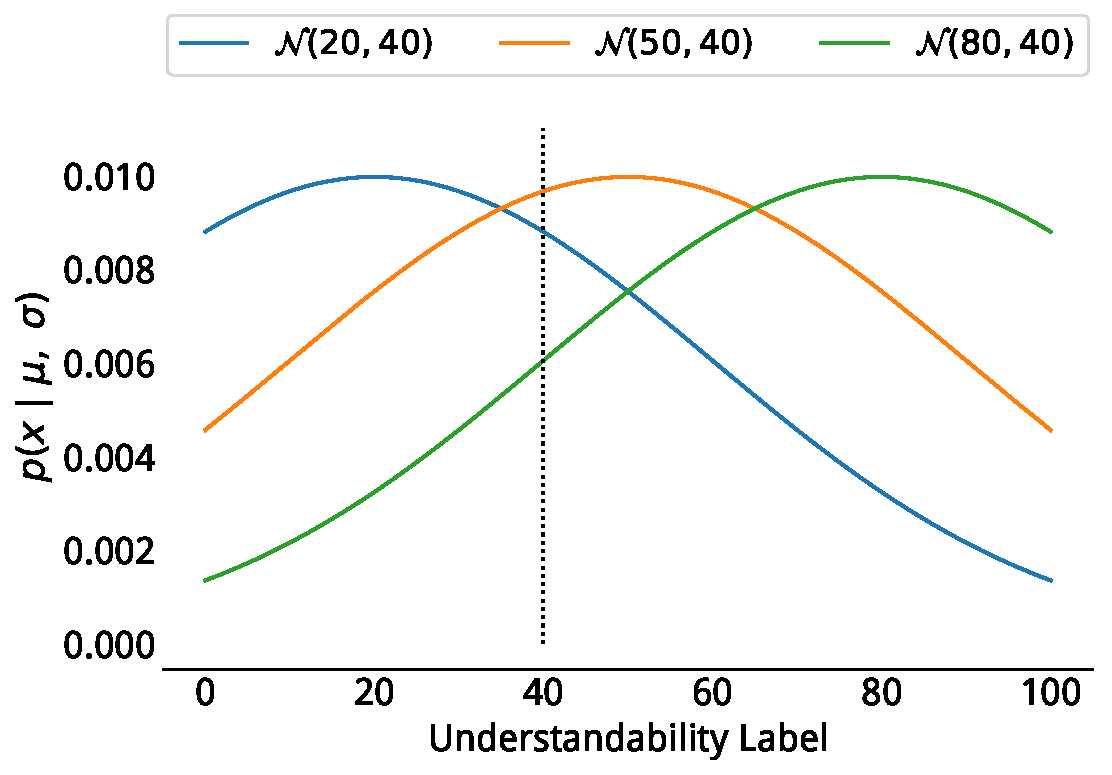
\includegraphics[width=0.30\textwidth]{figs/gaussians}
    \vspace{-.2cm}
    \caption{Gaussian distribution for different $\mu$: higher $\mu$ generates higher understandability labels (harder documents were retrieved). Here, only documents with understandability lower than 40 are considered easy-to-understand. (Understandability threshold shown as dotted line). \vspace{-16pt}}
  \label{fig:gaussians}
\end{figure}


We calculated $uRBP$ (using UBIRE) and $MM_{RBP}$ for each synthetic system.
The average result of the synthetic runs is shown in Table~\ref{tab:simulations}. Each row shows the results of simulations with different values for $T$, i.e., different expected number of topical documents retrieved.
We varied $\mu$ which was used to create the understandability labels, and show the results for $\mu = 50, 40, 30$.
A smaller $\mu$ means that more understandable documents were retrieved. The results show that as the expected number of topical documents ($T$) increases, $RBP$ increases. Likewise, $uRBP$ increases, as it is bounded by topical relevance.
In turn, increasing $T$ has no effect on $RBP_u$, but increases $MM_{RBP}$, as it is also directly dependant on $RBP$. When the number of understandable documents retrieved is increased (i.e., $\mu$ decreased ), $RBP$ stays constant, as it does not measure how understandable documents are.
In turn, $uRBP$, $RBP_u$ and $MM_{RBP}$ increase. 
Those are the expected behaviour of the considered measures. % aforementioned metrics and only shows that our simulated runs produce sane results.

We further focused our attention to the results of specific experiments highlighted in blue and yellow in Table~\ref{tab:simulations}. These cases simulated an initial system S1 that exhibited the results in blue (condition $T=0.6$ and $\mathcal{N}(40,40)$) being modified to improve the understandability of retrieved documents ($\mathcal{N}(30,40)$) at the expenses of topicality ($T=0.5$), producing a new system S2. The effectiveness of S2 is highlighted in yellow. 

If $RBP$ and $uRBP$ were used to decide whether S2 should be preferred over the initial system S1, then S2 would be discarded and S1 preferred, as S2 produced a $18\%$ reduction in $RBP$ and a $13\%$ reduction in $uRBP$. With these results, an IR researcher would conclude that the modifications in S2 did not pay off.

If $MM_{RBP}$ was used instead, the IR researcher would have been able to gain more insights about system effectiveness and the trade-off between understandability and topicality. To use $MM_{RBP}$, $RBP_t$ ($=RBP$) and $RBP_u$ needed to be computed. Between S1 and S2, there was a decrease in $RBP_t$ of $18\%$; but conversely $RBP_u$ increased by $24\%$: this clearly allows to gauge the trade-off between topicality and understandability. 

When $RBP$ and $uRBP$ were combined within $MM_{RBP}$, if both dimensions were given equal weight, then systems S1 and S2 obtained the same $MM_{RBP}$. Note that $MM$ can be adapted to specific circumstances: if topicality was more important than understandability, then the weights of each dimension would have been changed accordingly in the harmonic mean computation. 

%%%%%%%%%%%%%%%%%%%%%%%%%%%%%%%%%%%%%%%%%%%%%%%%%%%%%%%%%%%%%%%%%%%%%%%%%%%%%%%%%%%%%%%%%%%%%%%%%%%%%%%%%%%%%%%%%%%%%%%%%%%%%%%%
%%%%%%%%%%%%%%%%%%%%%%%%%%%%%%%%%%%%%%%%%%%%%%%%%%%%%%%%%%%%%%%%%%%%%%%%%%%%%%%%%%%%%%%%%%%%%%%%%%%%%%%%%%%%%%%%%%%%%%%%%%%%%%%%
%%%%%%%%%%%%%%%%%%%%%%%%%%%%%%%%%%%%%%%%%%%%%%%%%%%%%%%%%%%%%%%%%%%%%%%%%%%%%%%%%%%%%%%%%%%%%%%%%%%%%%%%%%%%%%%%%%%%%%%%%%%%%%%%
%%%%%%%%%%%%%%%%%%%%%%%%%%%%%%%%%%%%%%%%%%%%%%%%%%%%%%%%%%%%%%%%%%%%%%%%%%%%%%%%%%%%%%%%%%%%%%%%%%%%%%%%%%%%%%%%%%%%%%%%%%%%%%%%


%\section{Non-Simulated Experiments}
\section{Rank Correlations} %across Systems and Measures}
\label{sec:clef}


\begin{table}[t]
    \centering
    \caption{Kendall-$\tau$ correlation for systems participating in CLEF eHealth 2015 and 2016.     \vspace{-6pt}
    %uRBP merges the understandability labels with the default RBP using UBIRE framework. $H_{RBP}$ is the weighted geometric mean of RBP and $RBP_u$: the former measures only topicability and the latter, only understandability.
    }
    \label{tab:kendall}
    %
    \resizebox{0.45\textwidth}{!}{ %
    \begin{tabular}{@{}l|llll|llll@{}}
        \toprule
                  & \multicolumn{4}{c}{\textbf{CLEF 2015}} & \multicolumn{4}{c}{\textbf{CLEF 2016}} \\ \cmidrule{2-9} 
                  & RBP     & uRBP    & $RBP_u$   & $H_{RBP}$  & RBP     & uRBP    & $RBP_u$   & $H_{RBP}$  \\ 
                  RBP           & 1.000   & 0.901   & 0.483    & 0.843   & 1.000   & 0.948   & 0.497    & 0.850   \\
                  uRBP          & 0.901   & 1.000   & 0.563    & 0.901   & 0.948   & 1.000   & 0.456    & 0.866   \\
                  $RBP_u$       & 0.483   & 0.563   & 1.000    & 0.610   & 0.497   & 0.524   & 1.000    & 0.633   \\
                  $H_{RBP}$     & 0.843   & 0.901   & 0.610    & 1.000   & 0.850   & 0.866   & 0.633    & 1.000   \\ 
        \bottomrule
    \end{tabular}
    } % end resizebox
    \vspace{-18pt}
\end{table}






\section{Conclusion}
\label{sec:conclusion}

In this paper, we proposed a new framework to evaluate multi-dimensional search engines called $H$.
We compare $H$ to UBIRE, a framework that has been used in recent years to evaluate systems in the consumer health search domain.
Our experiments demonstrated that while $H$ correlated well with UBIRE (i.e. they have equivalent power to rank and distinguish good systems),
$H$ has the advantage of allowing experimenters to easily understand how well their systems are working.


%\section{Preprocessing Pipelines and Heuristics}

%\section{Which Preprocessing Approach To Prefer}
Next, we studied the influence of the preprocessing of Web pages on the estimation of understandability when using the methods evaluated in the previous section. We did so by comparing the combination of a number of pre-processing pipelines, heuristics and understandability estimation methods with human assessments of web page understandability. 
Our experiments extended those by Palotti et al.~\cite{palotti15}, who did only evaluate surface level readability formulas and did not compare their results against human assessments. 

We employed the same three approaches used in Palotti et al.~\cite{palotti15} to extract the content of a Web page from the HTML source: BeautifulSoap~\cite{bs4} (\textit{Naive}), which just naively removes HTML tags, Boilerpipe~\cite{kohlschutter10} (\textit{Boilerpipe - Boi}) and Justext~\cite{jan11} ({Justext - Jst}), which eliminate boilerplate text together with HTML tags. 
Their data analysis highlighted that the text in HTML tags often missed a correct punctuation mark and thus the text extracted from HTML fields like titles, menus, tables and lists could be interpreted as many short sentences or few very long sentences, depending on whether a period was forced at the end of fields/sentences. We thus implemented the same two heuristics to deal with this: \textit{ForcePeriod - FP} and \textit{DoNotForcePeriod - DNFP}. The \textit{ForcePeriod - FP} heuristics forced a period at the end of each extracted HTML field; while the \textit{DoNotForcePeriod - DNFP} did not. 


\section{Evaluation of Preprocessing Pipelines and Heuristics}
\label{sec:which_preprocessing}
Results from these experiments are shown in Figure~\ref{fig:boxplot_corr_docs} (top: CLEF 2015; bottom: CLEF 2016). For each category of methods and combination of preprocessing and heuristics, we reported their variability in Spearman rank correlation with the human assessments\footnote{Results for Pearson and Kendall correlation measures are reported in the online appendix, but showed similar trends.}. We further reported summary results across all understandability assessments methods and sentence ending heuristics for each of the preprocessing pipelines. Finally, we also reported the inter-assessor correlation (last box) when multiple assessors provided judgements about the understandability of Web pages (see Section~\ref{sec:data} for details about this data). This provided an indication of the range of variability and subjectiveness when assessing understandability, along with the highest correlation we measured between human assessors. 

We first examined the correlations between human assessments and readability formulas. We found that the \textit{Naive} preprocessing resulted in the lowest correlations, regardless readability formula and heuristics (although \textit{DoNotForcePeriod} performed better than \textit{ForcePeriod}). Using Justext or Boilerplate resulted in higher correlations with human understandability assessments, and the \textit{ForcePeriod} heuristic was shown to be better than the other. These results confirm the speculations of Palotti et al.~\cite{palotti15}: they found these settings to produce lower variances in understandability estimations and thus hypothesise they were better suited to the task.

Overall, among readability formulas, the best results (highest correlations) were obtained by SMOG and Dale-Chall Index (see Table~\ref{tab:top_corr_metrics}). Although no single setting outperformed the others in both collections, we found that the use of CLI and FRE with \textit{Justext} provided the most stable results across the collections, with correlation coefficients as high as the best ones in both collections.
These results confirmed the advice put forward by Palotti et al.~\cite{palotti15}, i.e. if using readability measures, then CLI should be preferred, along with an appropriate HTML extraction pipeline, regardless of the heuristic for sentence ending\footnote{We provide detailed plots to compare our results with Palotti's in the online appendix.}.

When considering methods beyond those based on readability formulas, we found that the highest correlations were archived by the regressors (MLR) and classifiers (MLC), independently of the preprocessing method used. For methods in these categories, correlations were only marginally influenced by preprocessing and heuristics, with the exception for regressors on CLEF 2015 that did exhibit not negligible variances. \todo{I think the text is not clear here: need to discuss.} 

A common trend when comparing preprocessing pipelines, is that the Naive pipeline provided the weakest correlations with human assessments for CLEF 2016, regardless of estimation methods and heuristics. This result however was not confirmed for CLEF 2015, where the Naive preprocessing did negatively influence correlations for the readability formula category (RF), but not for other categories, although it was generally associated with larger variances. 


%For that, we present in Figure~\ref{fig:boxplot_corr_docs} the box plot of Spearman rank correlation metric divided by preprocessing alternative for CLEF eHealth 2015 and 2016\footnote{Due to space limitation, additional plots with Pearson and Kendall correlations are available online at \url{XYZ}.}.
%Figures~\ref{fig:boxplot_corr_docs_2015} and~\ref{fig:boxplot_corr_docs_2016} the box plot of different correlation metrics divided by preprocessing alternative for CLEF eHealth 2015 and 2016. 
%For instance, the very first box plot in the upper part of these figures shows the absolute Pearson's rank correlation of different readability metrics when using a combination of Naive and ForcePeriod as preprocessing steps.
%Boxes extend from the lower to upper quartile values of the data, with a line at the median. Whiskers extend from the box to show the range of the data. Flier points are those past the end of the whiskers, usually interpreted as outlier values.




%We also include in Figures~\ref{fig:boxplot_corr_docs_2015} and~\ref{fig:boxplot_corr_docs_2016} 
%We also include in Figure~\ref{fig:boxplot_corr_docs} boxes for the summary of the 3 preprocessing procedures to remove HTML, the use of HTML features, which is done without any preprocessing and the comparison with other human assessors. For CLEF eHealth 2015, we used as human assessments the additional assessments made by unpaid medical students and health consumers (see~\cite{palotti16b}), while for CLEF eHealth 2016 data, we randomly selected 100 pages that were assessed by another assessor. \mytodo{add at least another person doing assessments}.
%The correlations with human assessments provide important insights on how hard and subjective understandability assessments are.

\begin{figure*}[h!]
   \centering
   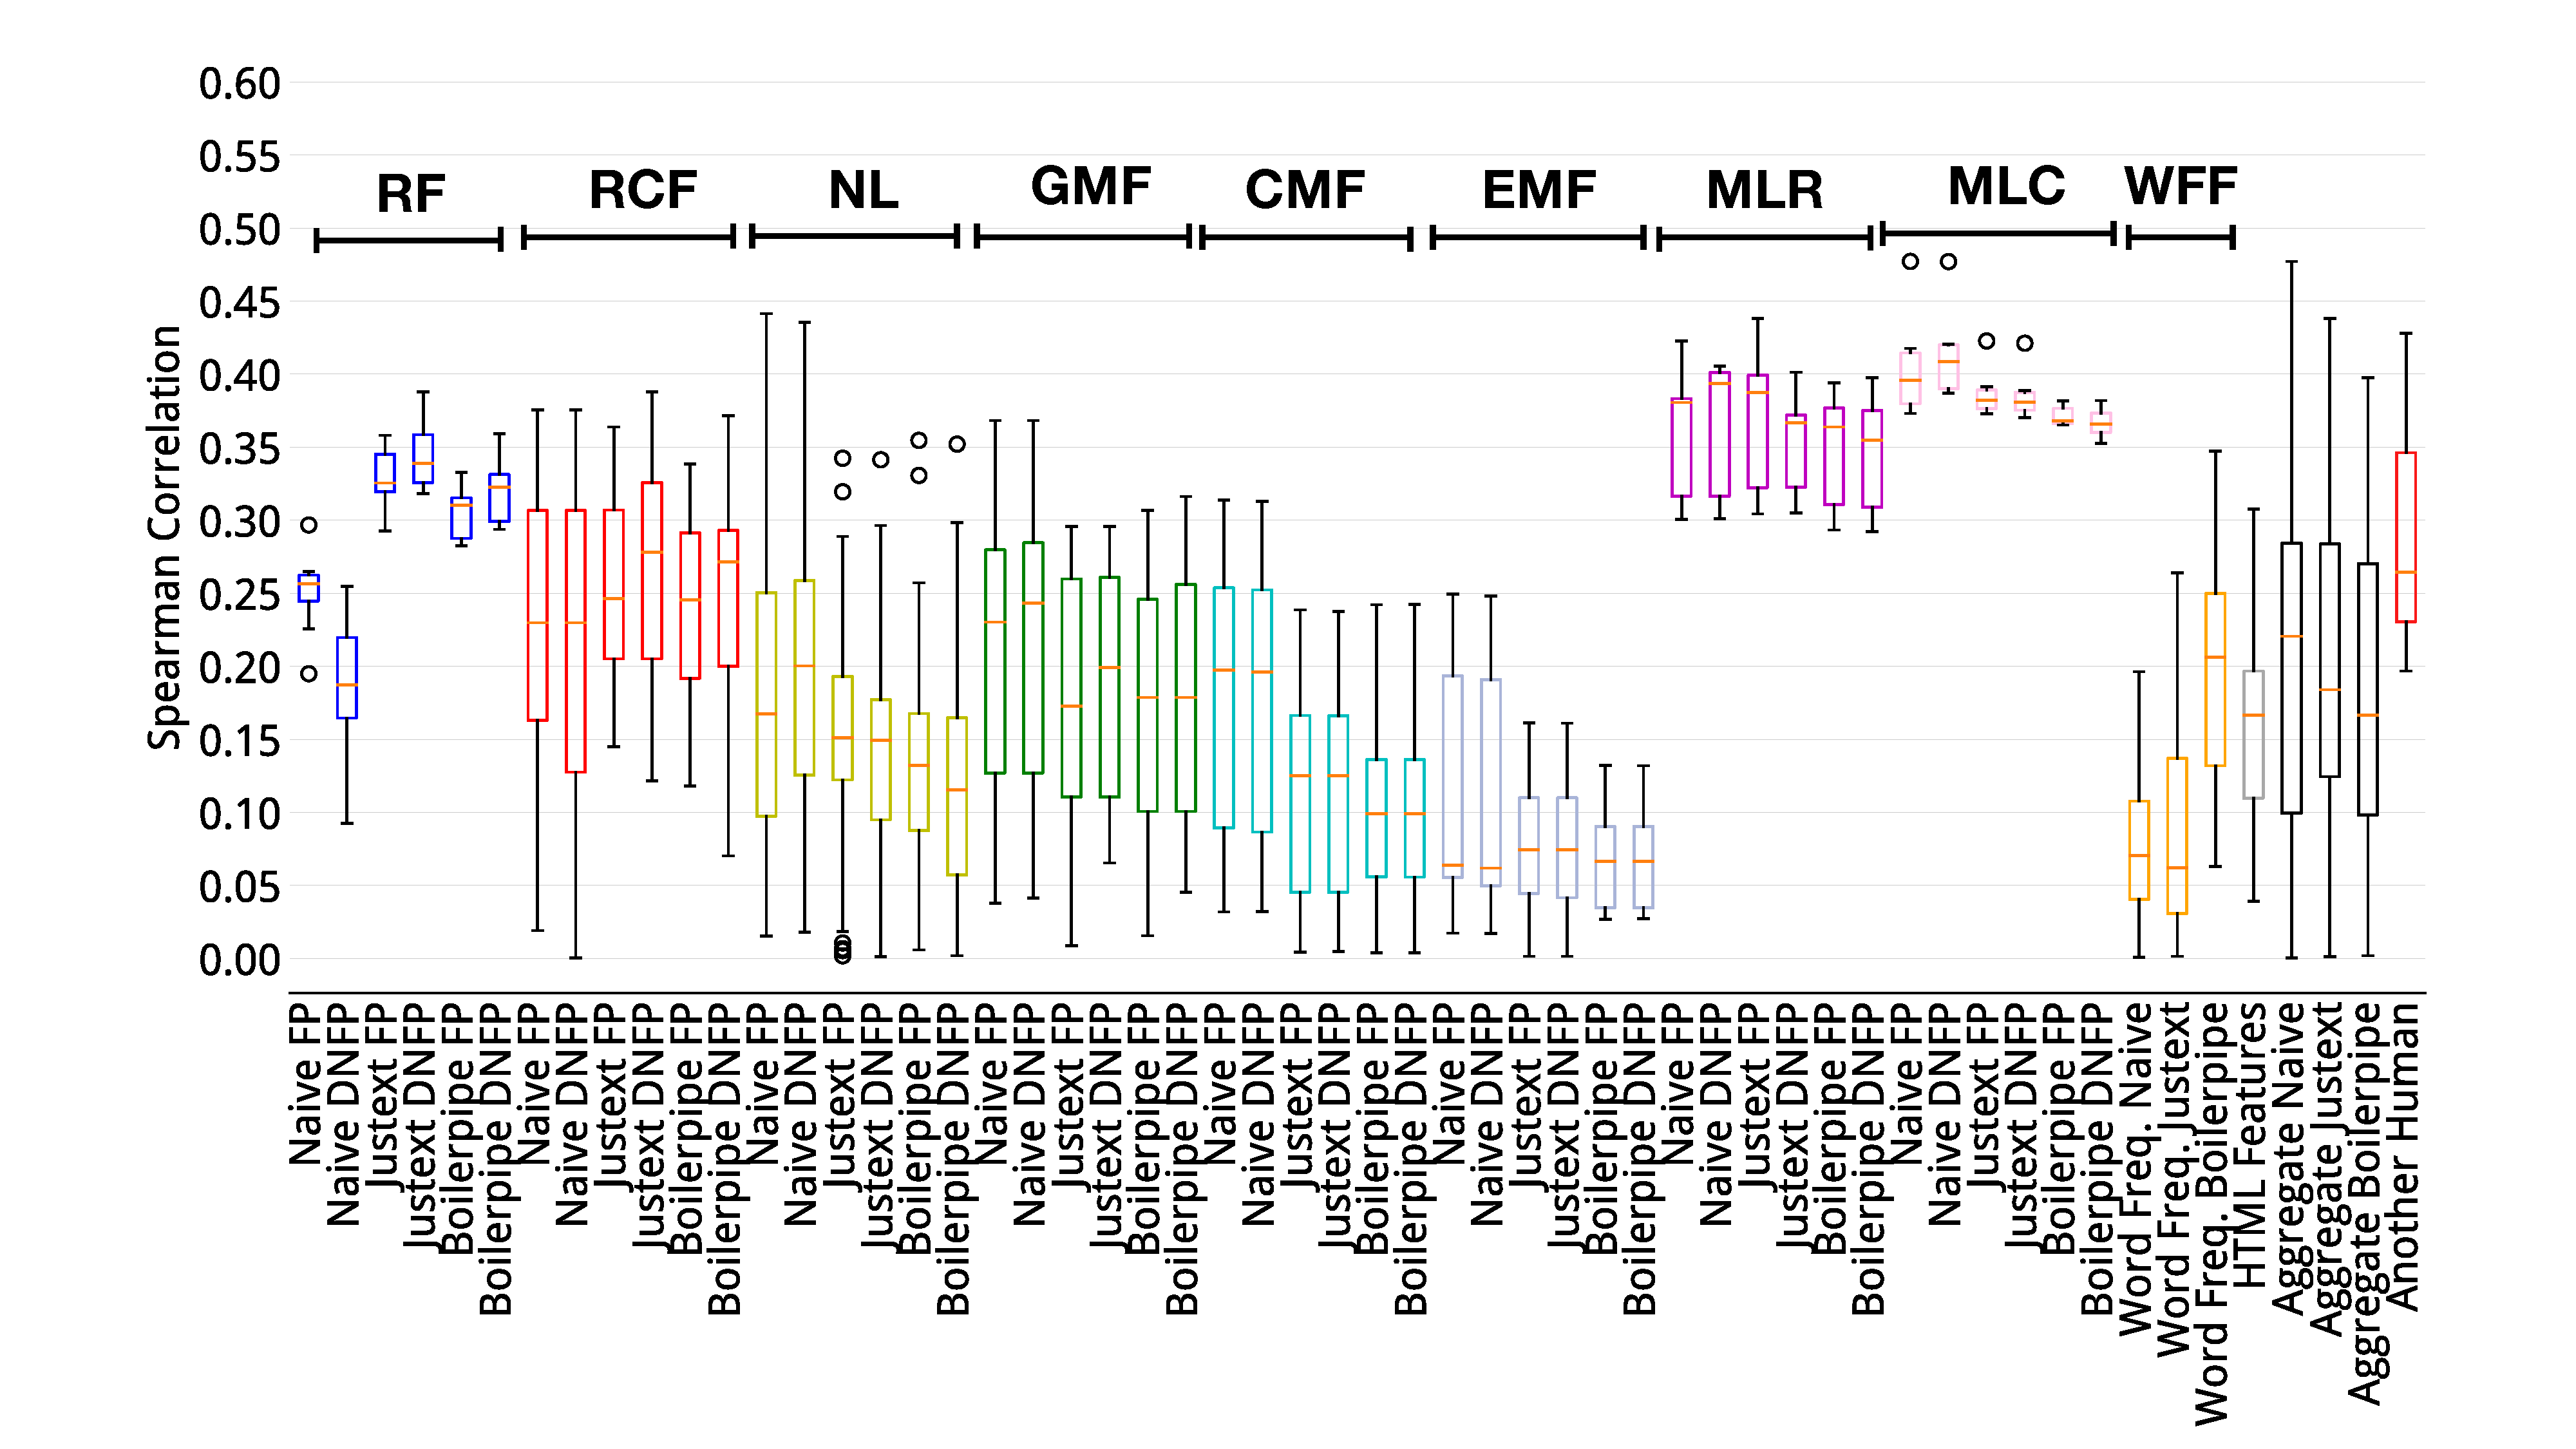
\includegraphics[width=0.80\textwidth]{graphics/box_spearman15_raw_values_mod}
   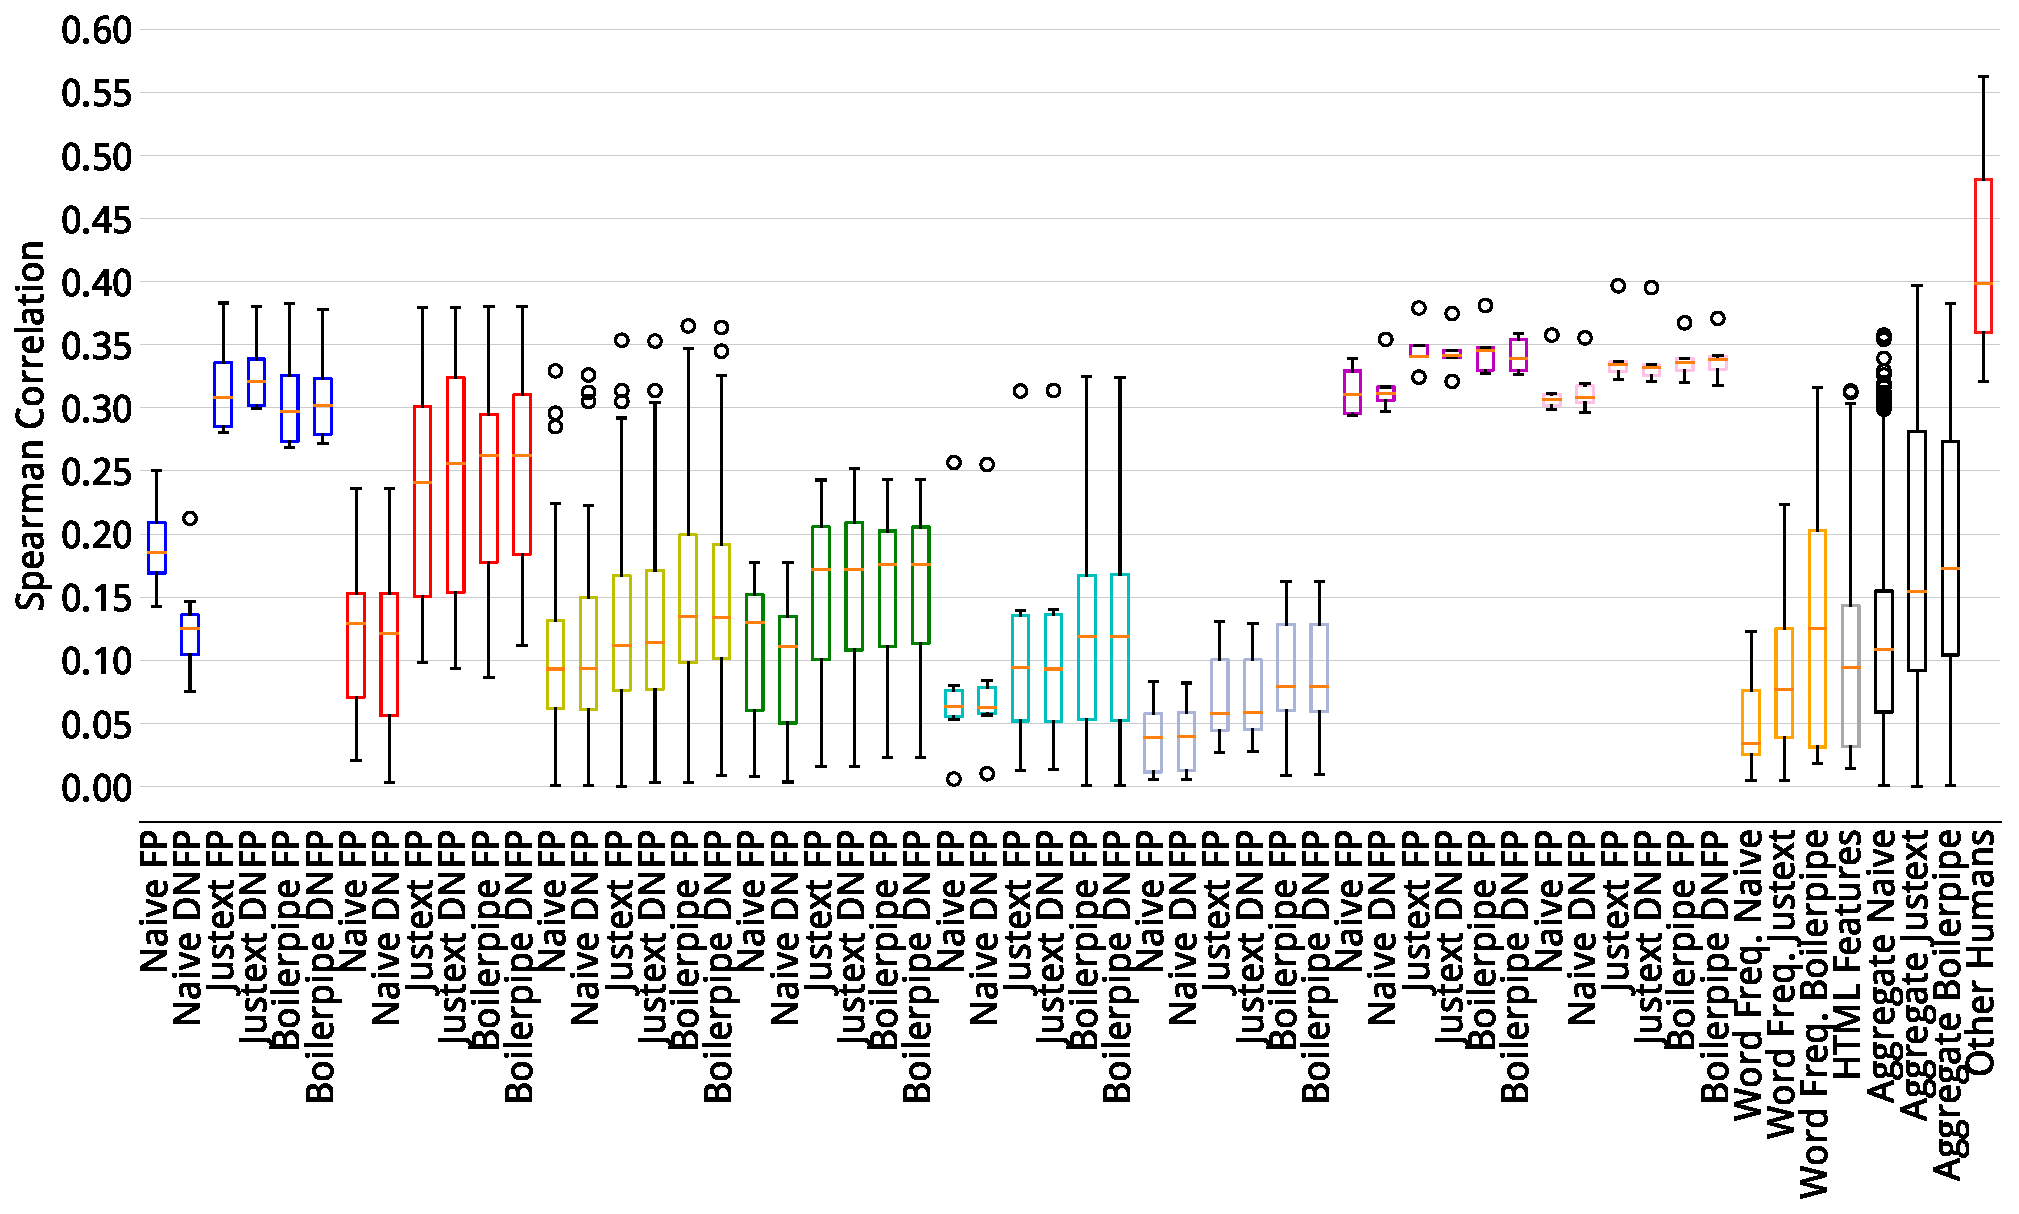
\includegraphics[width=0.80\textwidth]{graphics/box_spearman16_raw_values}
   %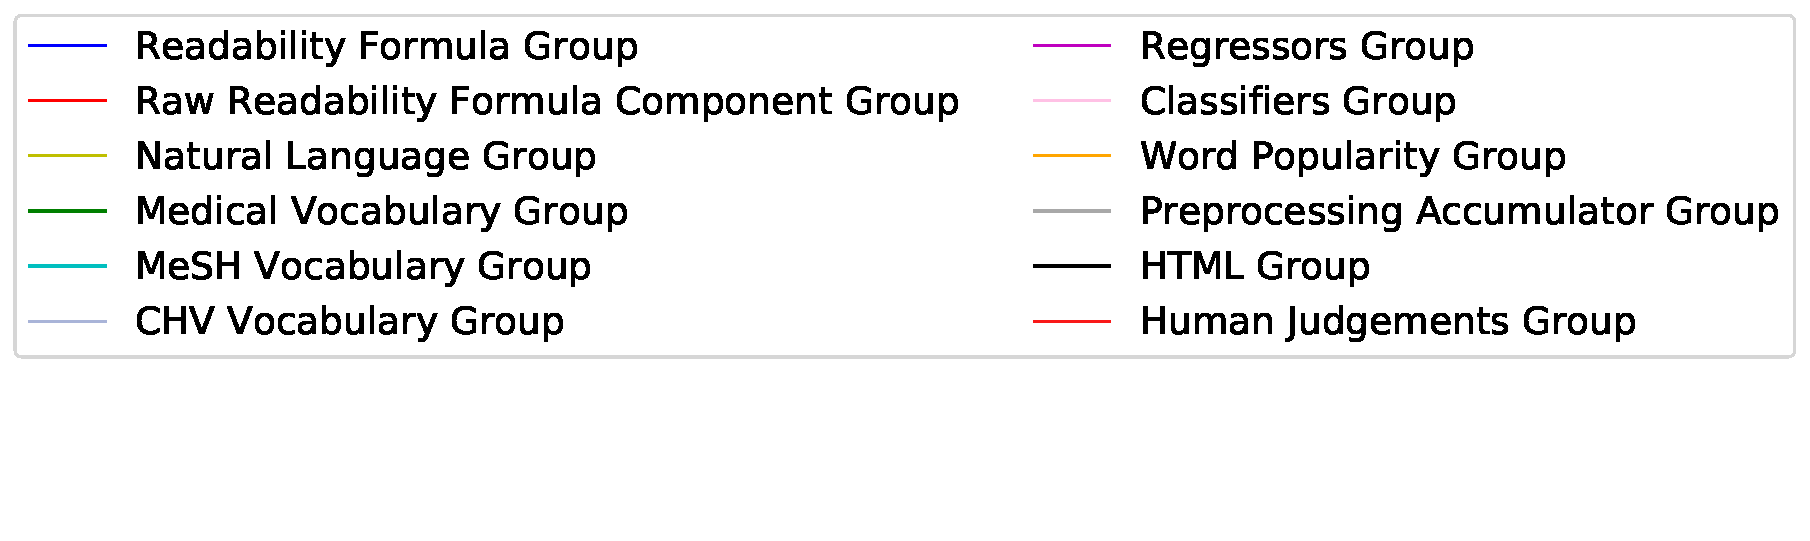
\includegraphics[width=0.7\textwidth]{graphics/legendCorr}
   \vspace{-1cm}
   \caption{Box plots divided by feature groups. Correlations are calculated using understandability labels from relevant documents assessed in CLEF eHealth 2015 (top) and 2016 (bottom).}
   \label{fig:boxplot_corr_docs}
\end{figure*}

%
%\begin{figure*}[th!]
%   \centering
%   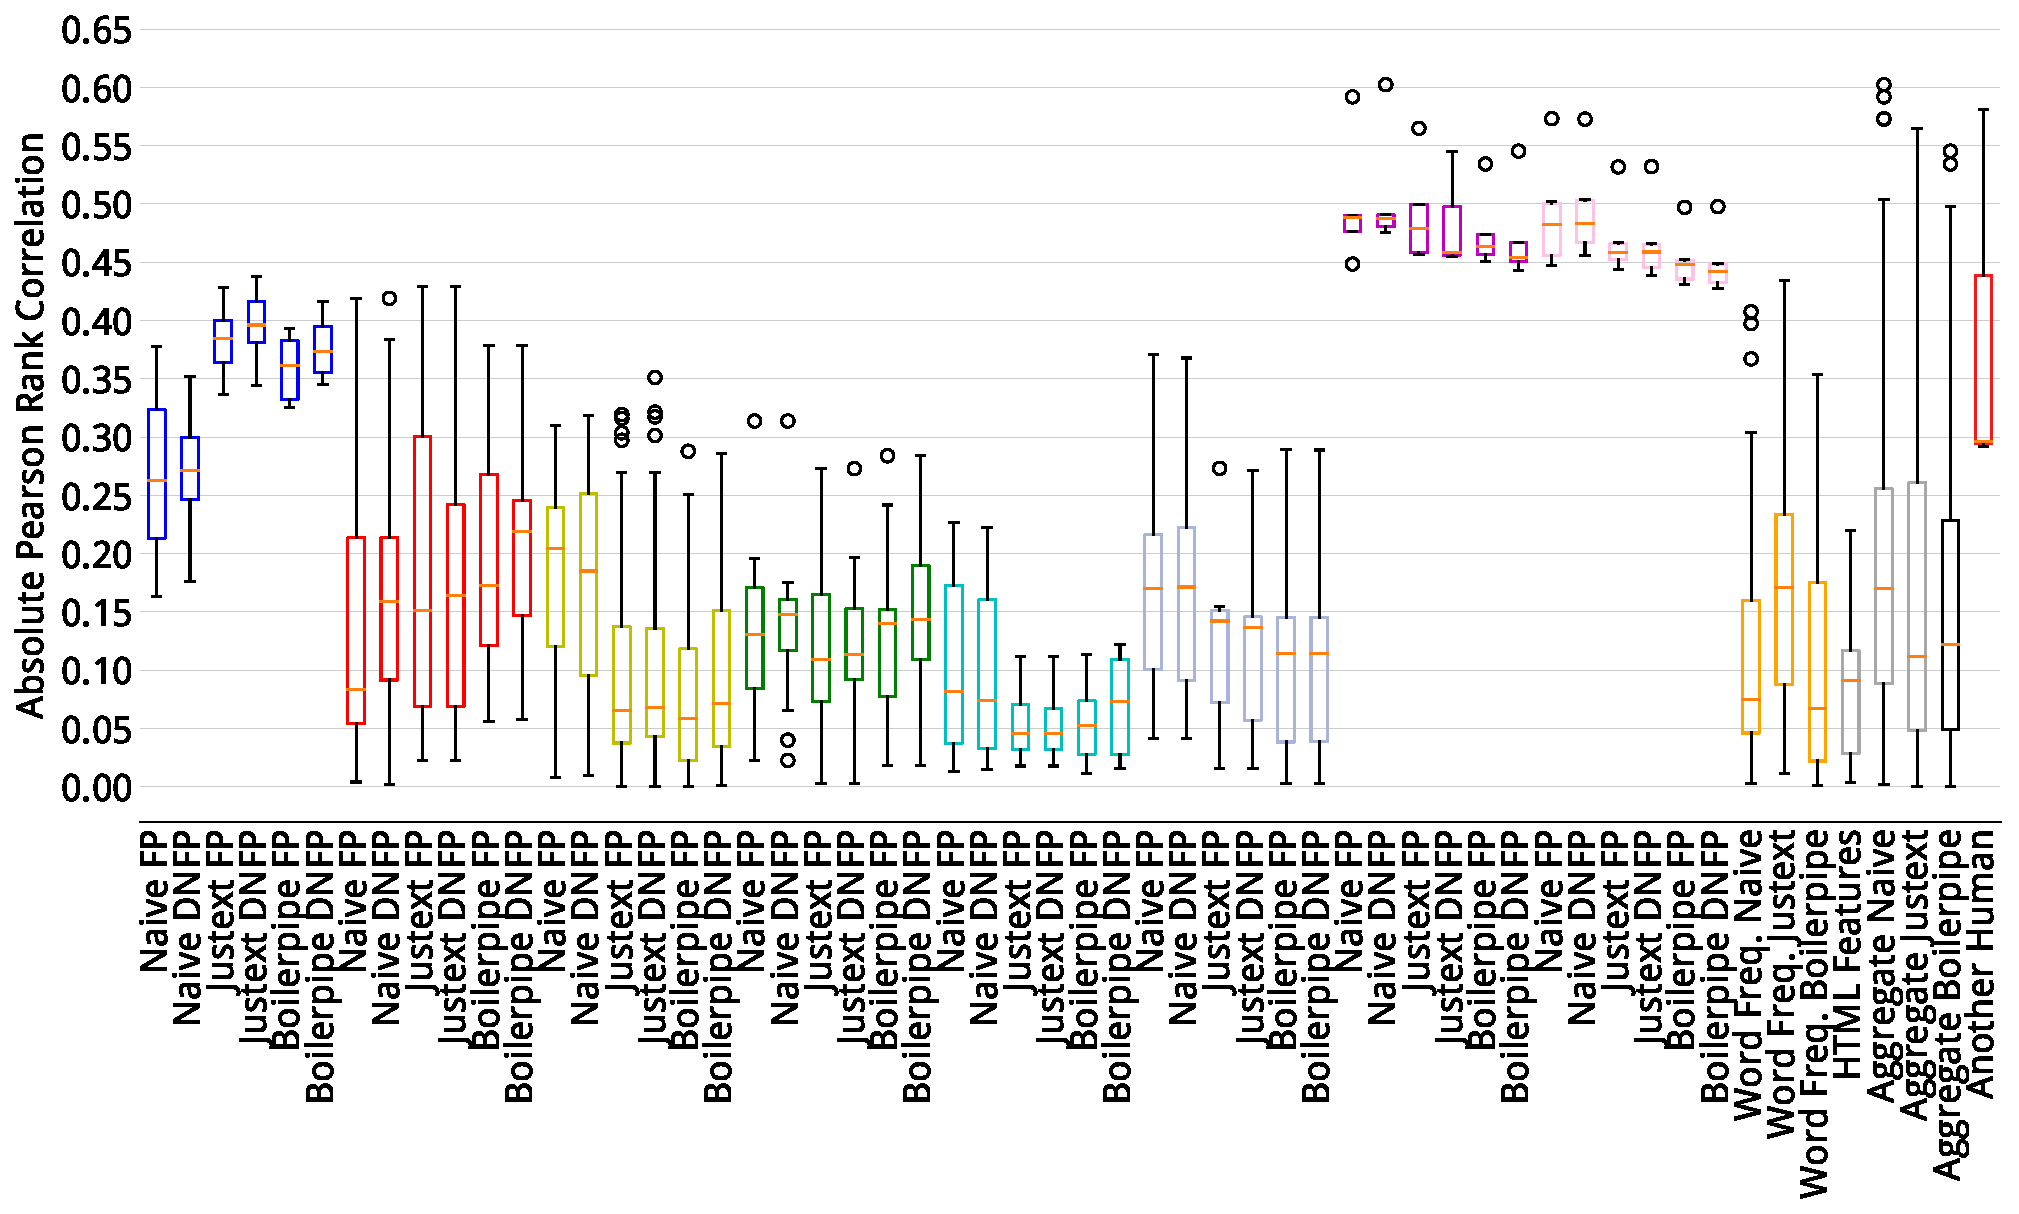
\includegraphics[width=0.90\textwidth]{graphics/box_pearson15_raw_values}
%   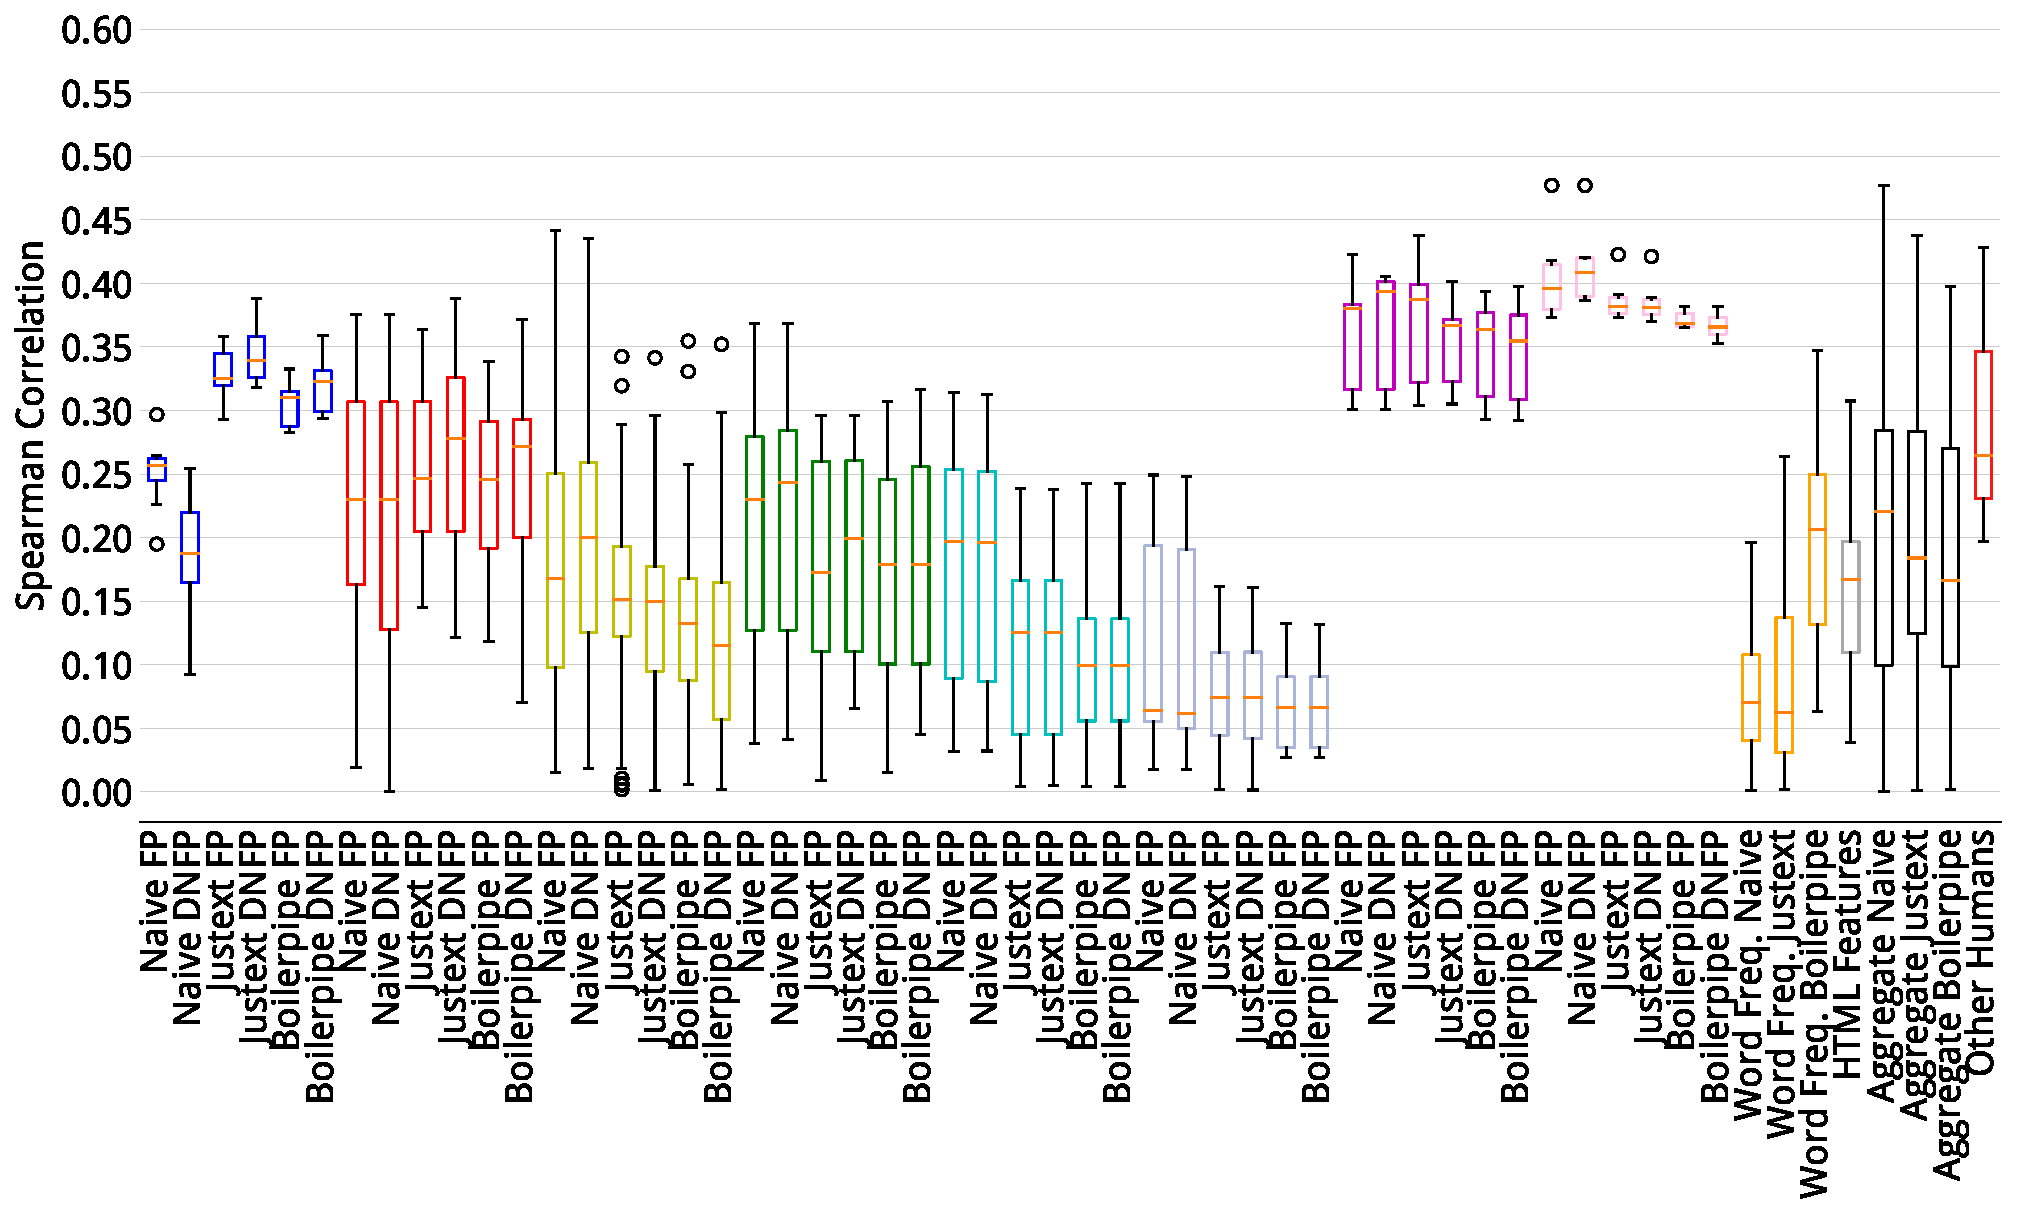
\includegraphics[width=0.90\textwidth]{graphics/box_spearman15_raw_values}
%   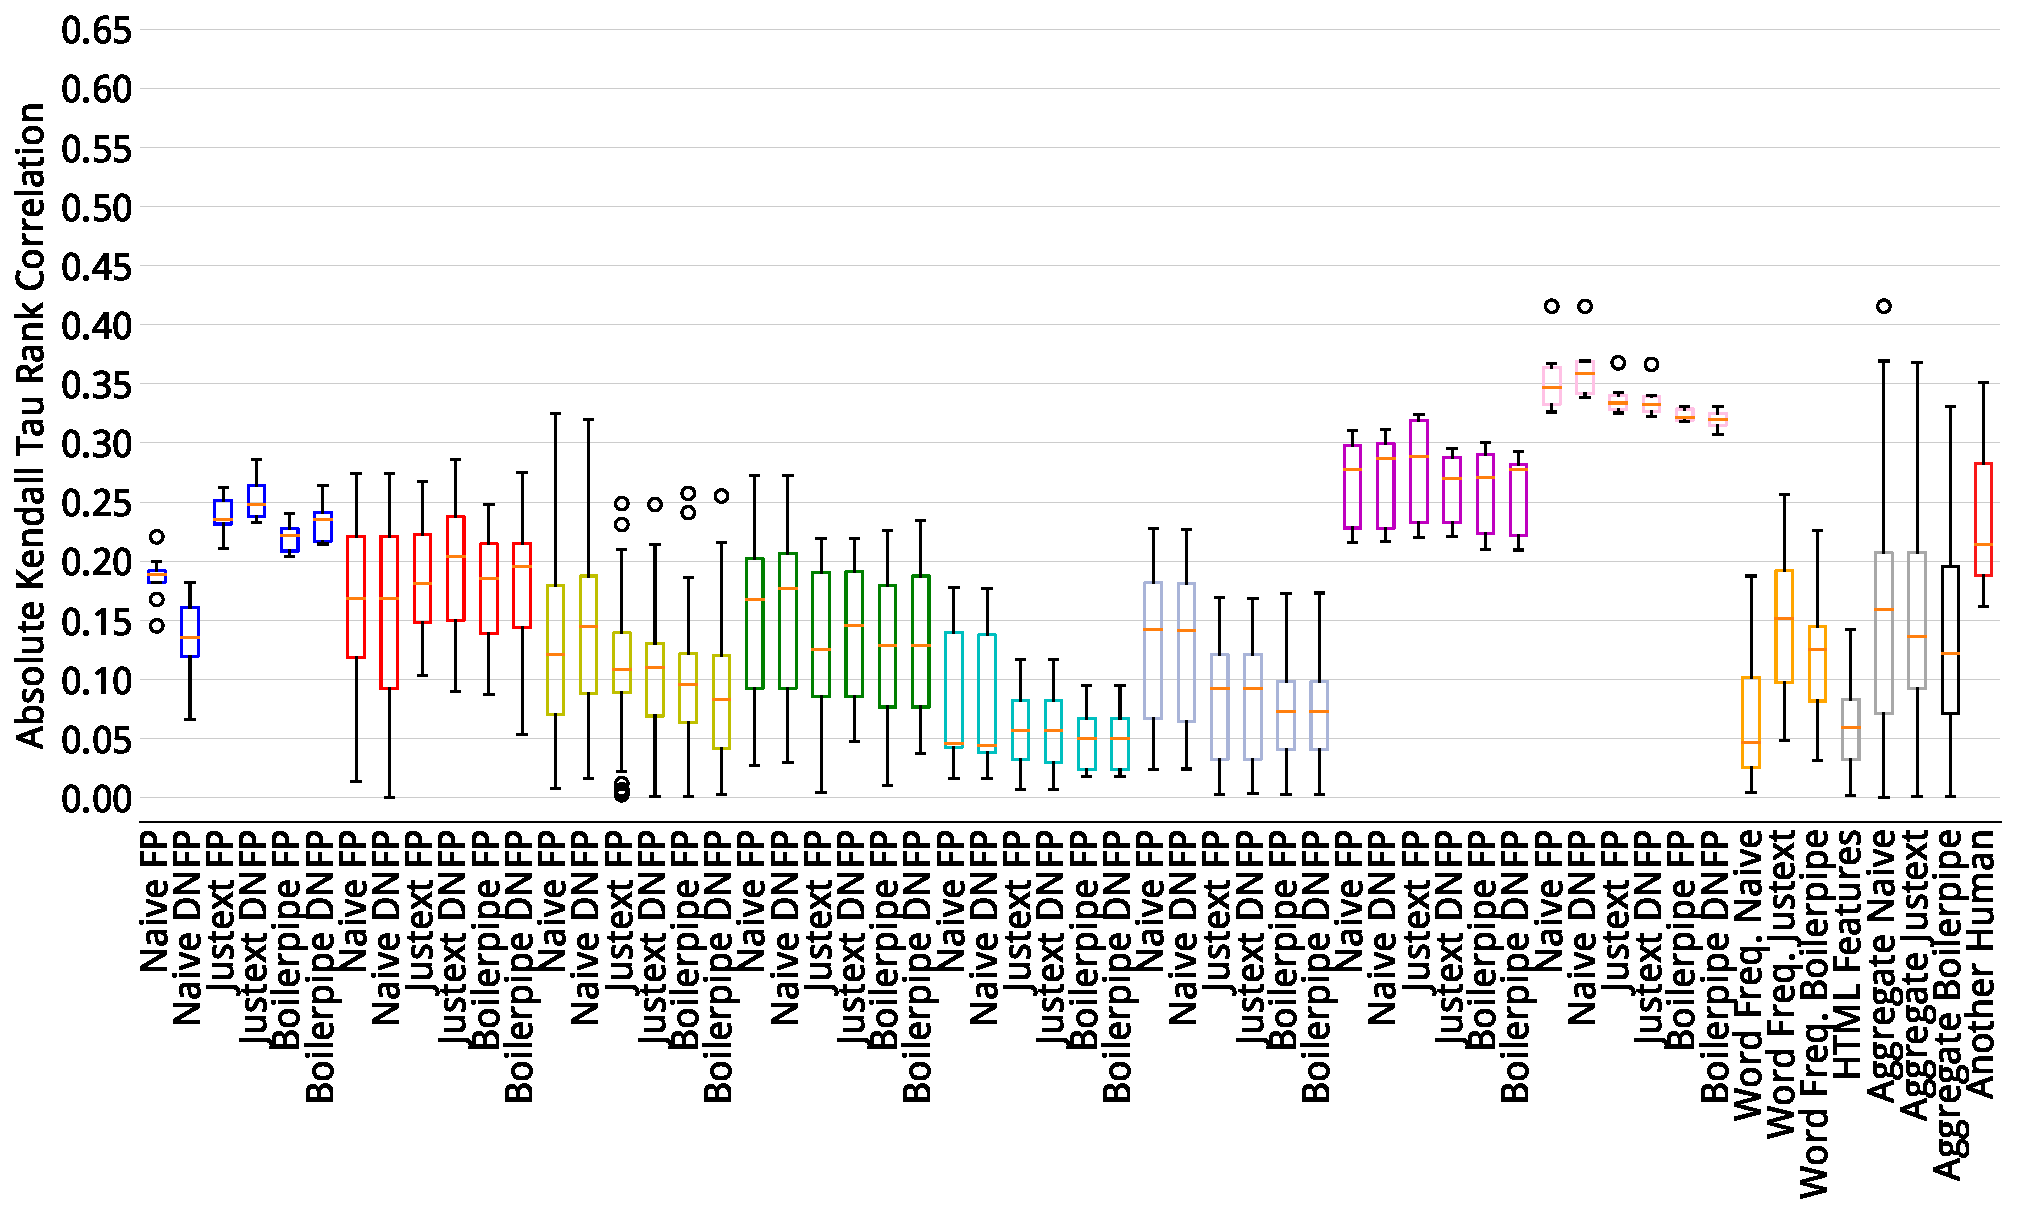
\includegraphics[width=0.90\textwidth]{graphics/box_kendalltau15_raw_values}
%   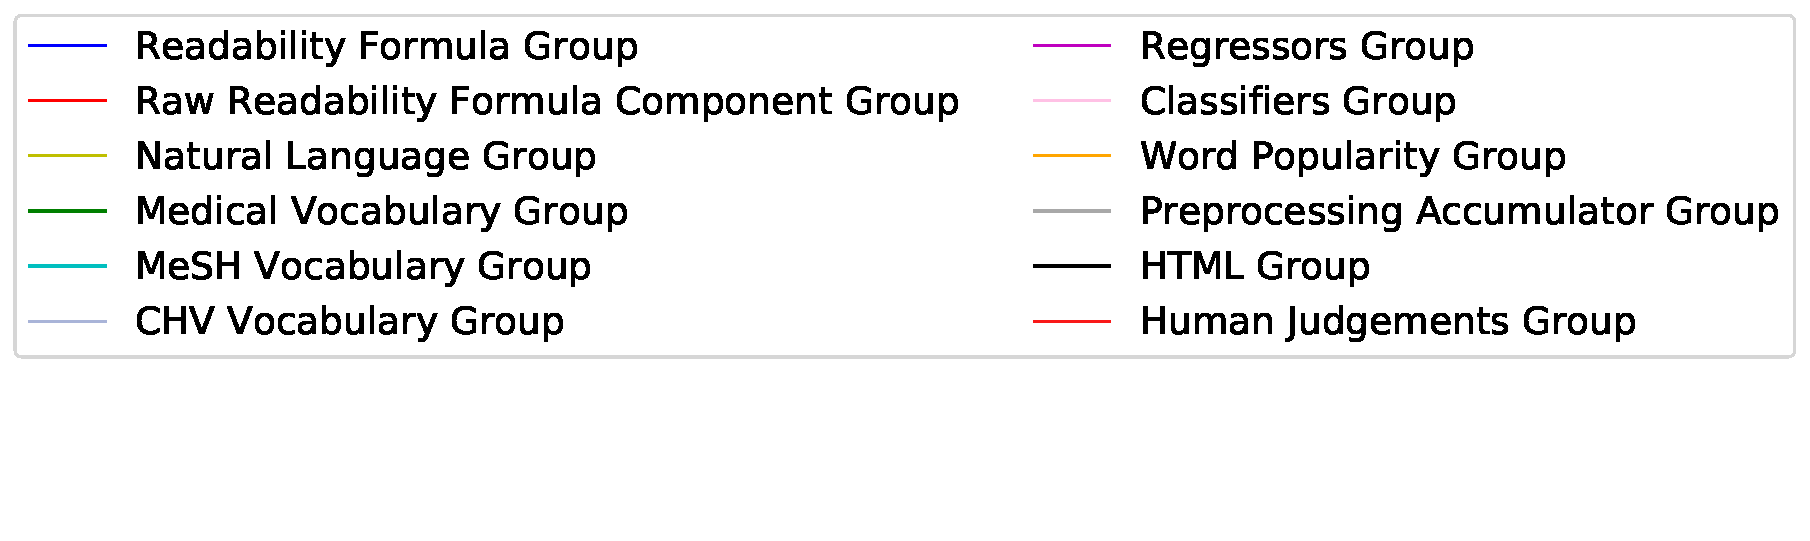
\includegraphics[width=0.65\textwidth]{graphics/legendCorr}
%   \caption{Box plots divided by feature groups. Correlations are calculated using understandability labels from relevant documents assessed in CLEF eHealth 2015}
%   \label{fig:boxplot_corr_docs_2015}
%\end{figure*}

%\begin{figure*}[th!]
%   \centering
%   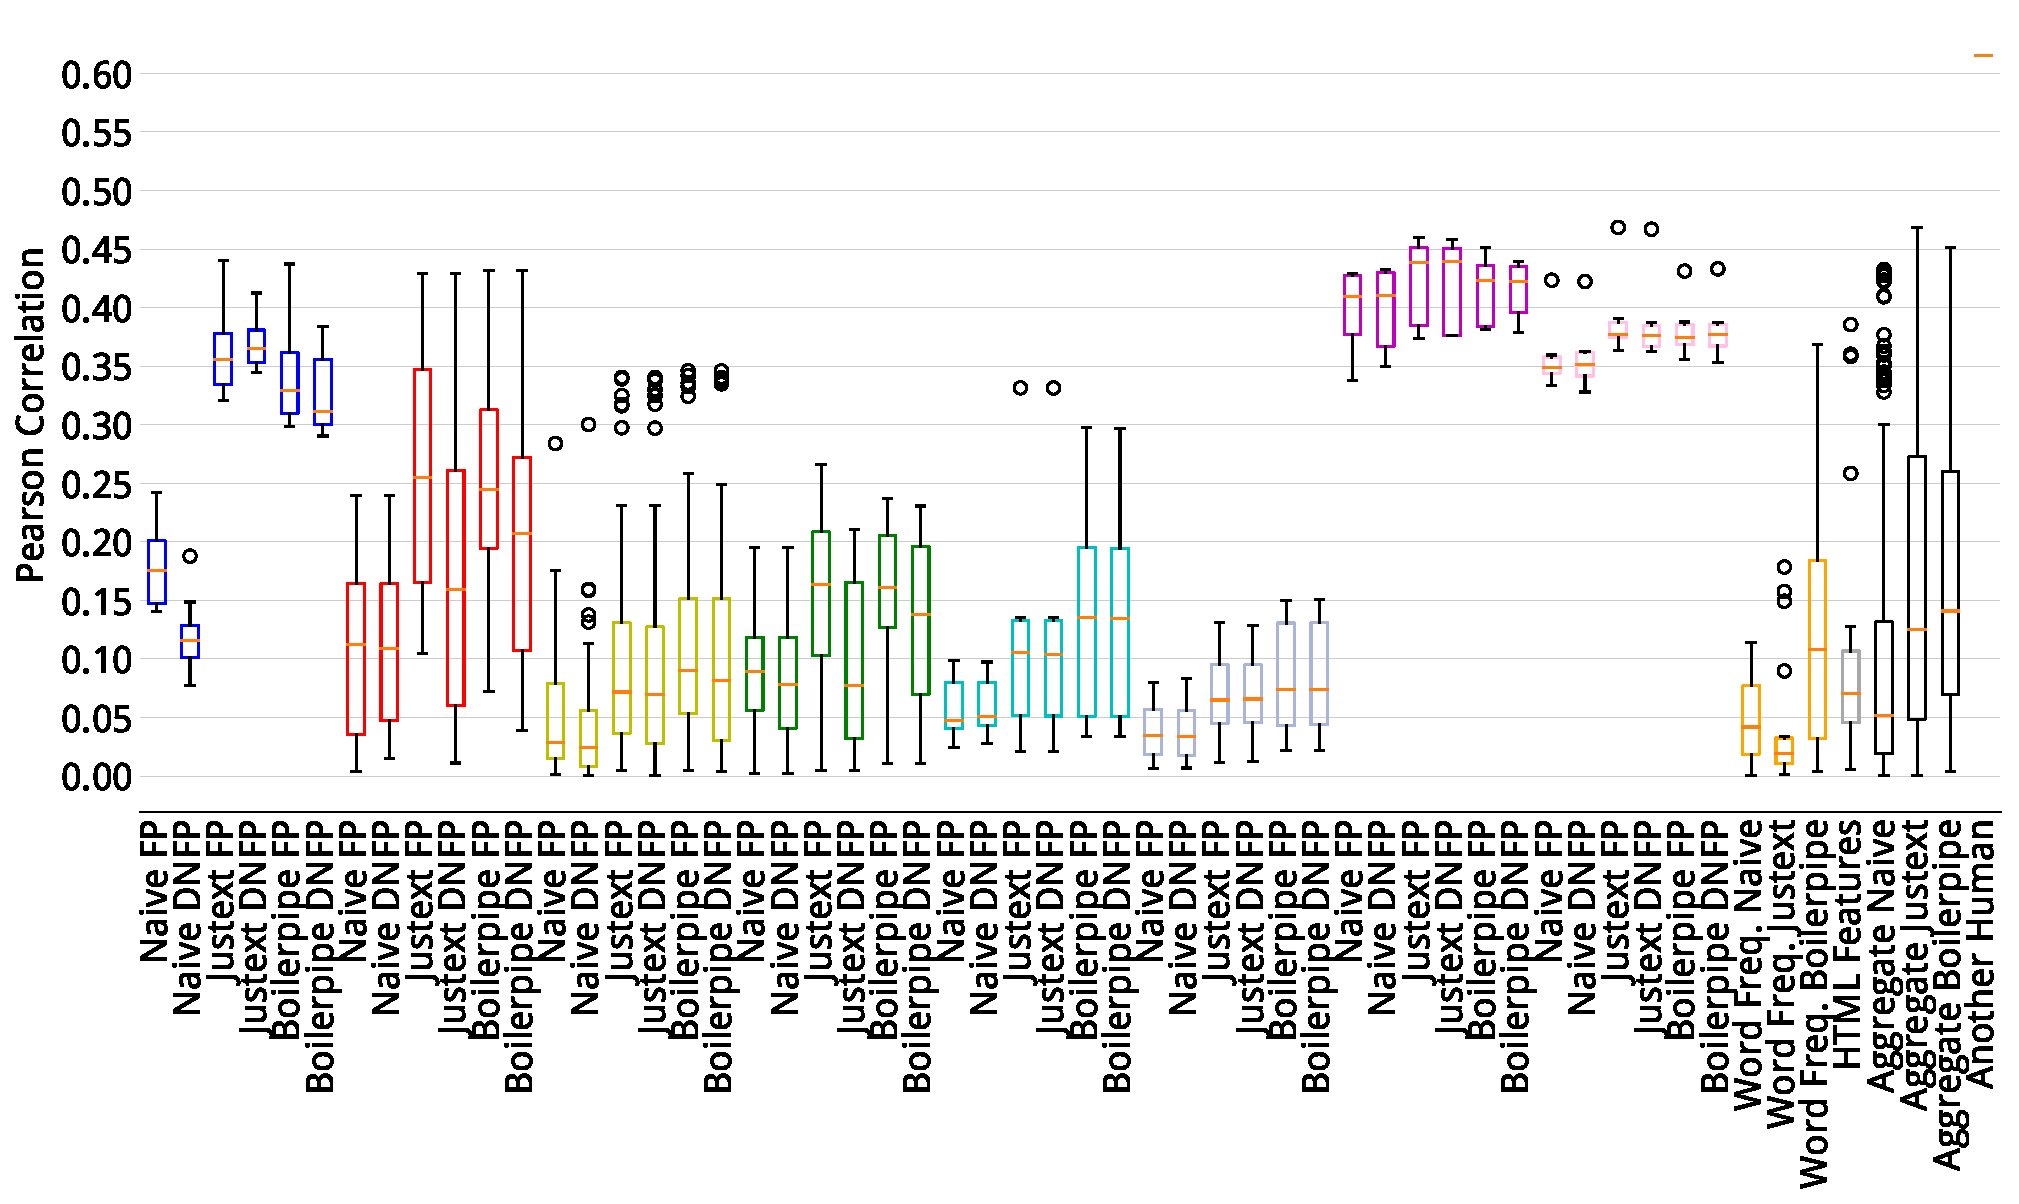
\includegraphics[width=0.90\textwidth]{graphics/box_pearson16_raw_values}
%   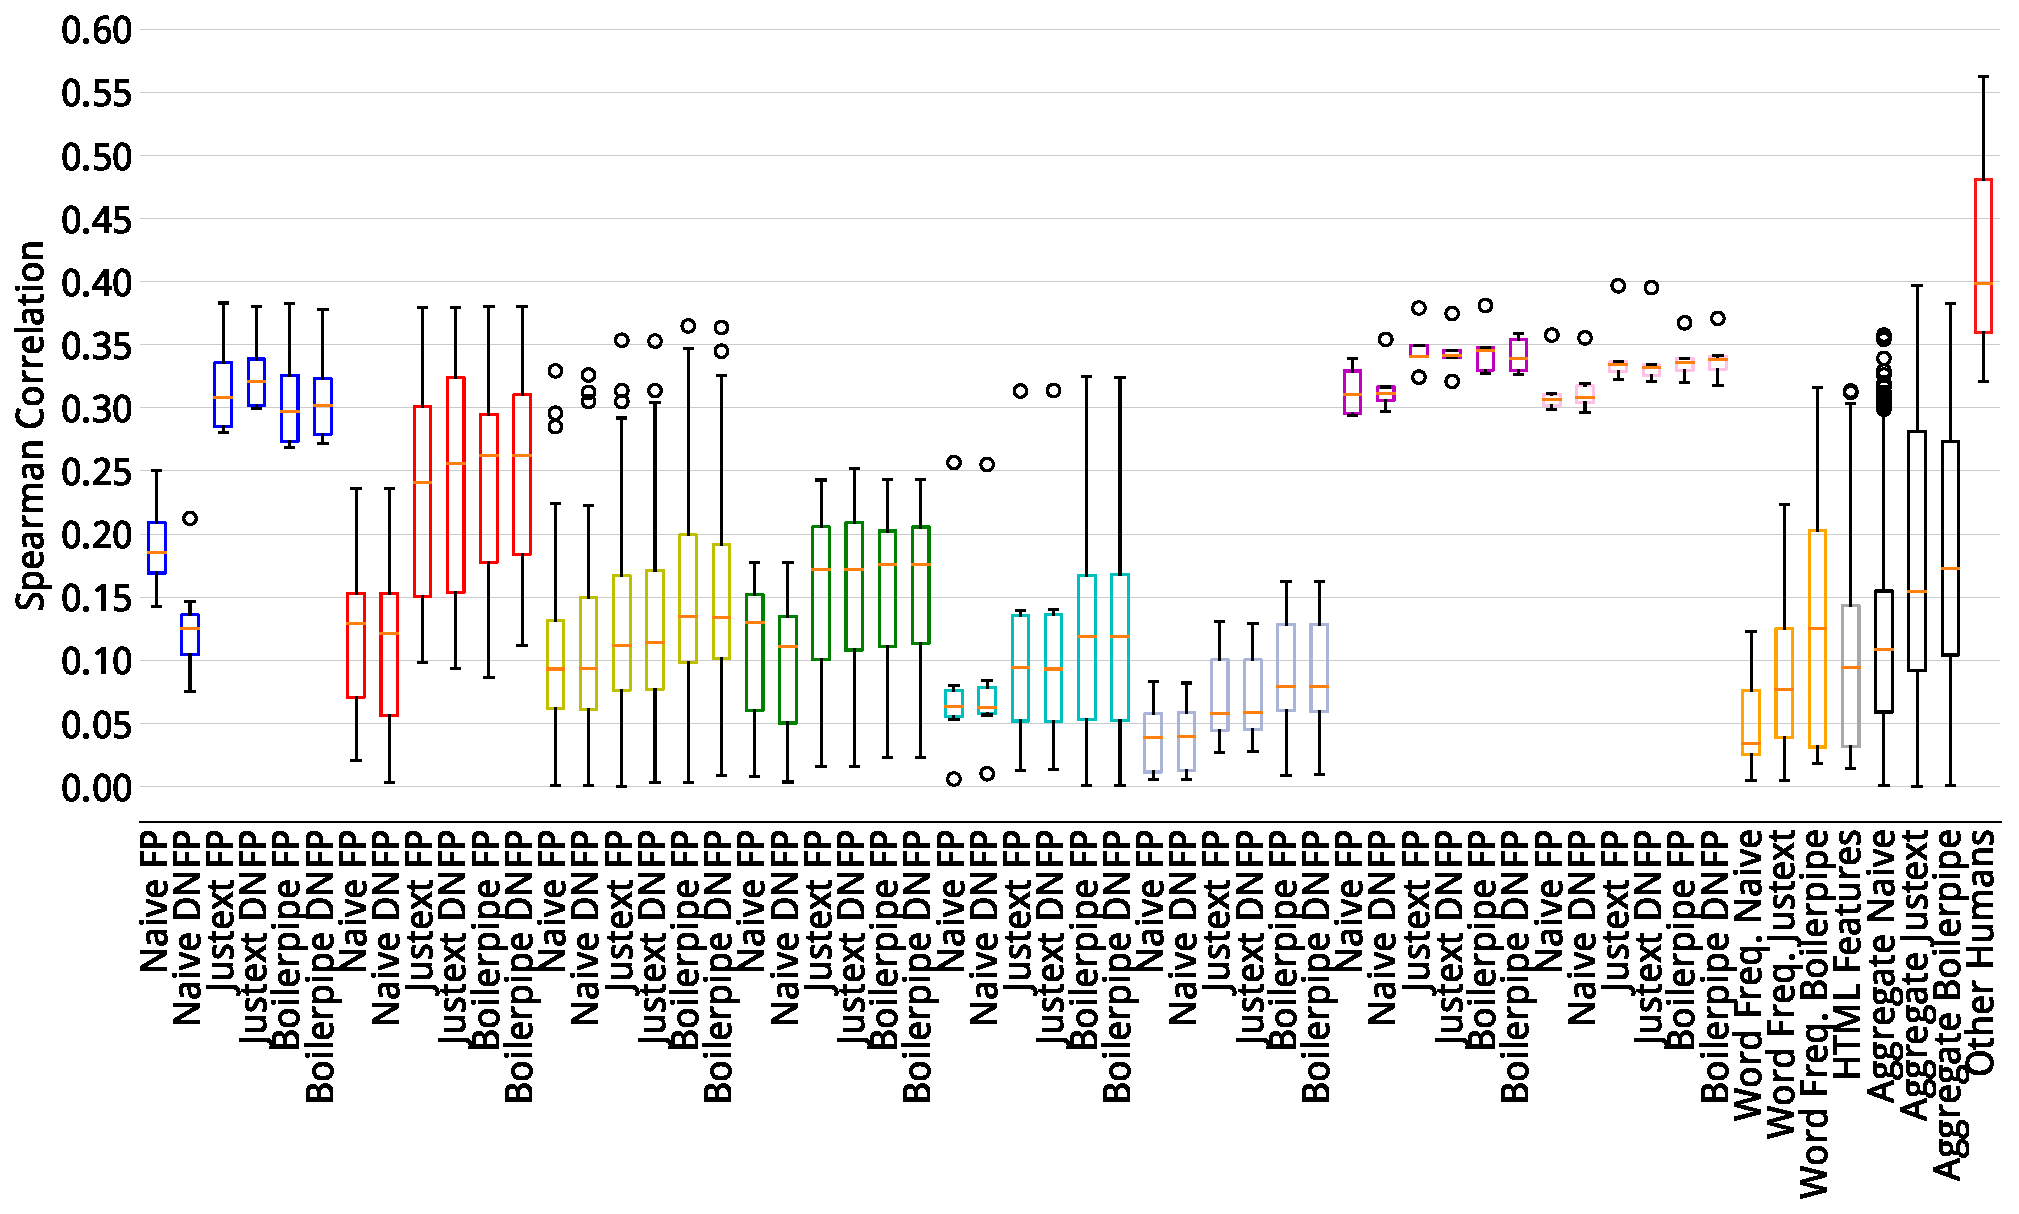
\includegraphics[width=0.90\textwidth]{graphics/box_spearman16_raw_values}
%   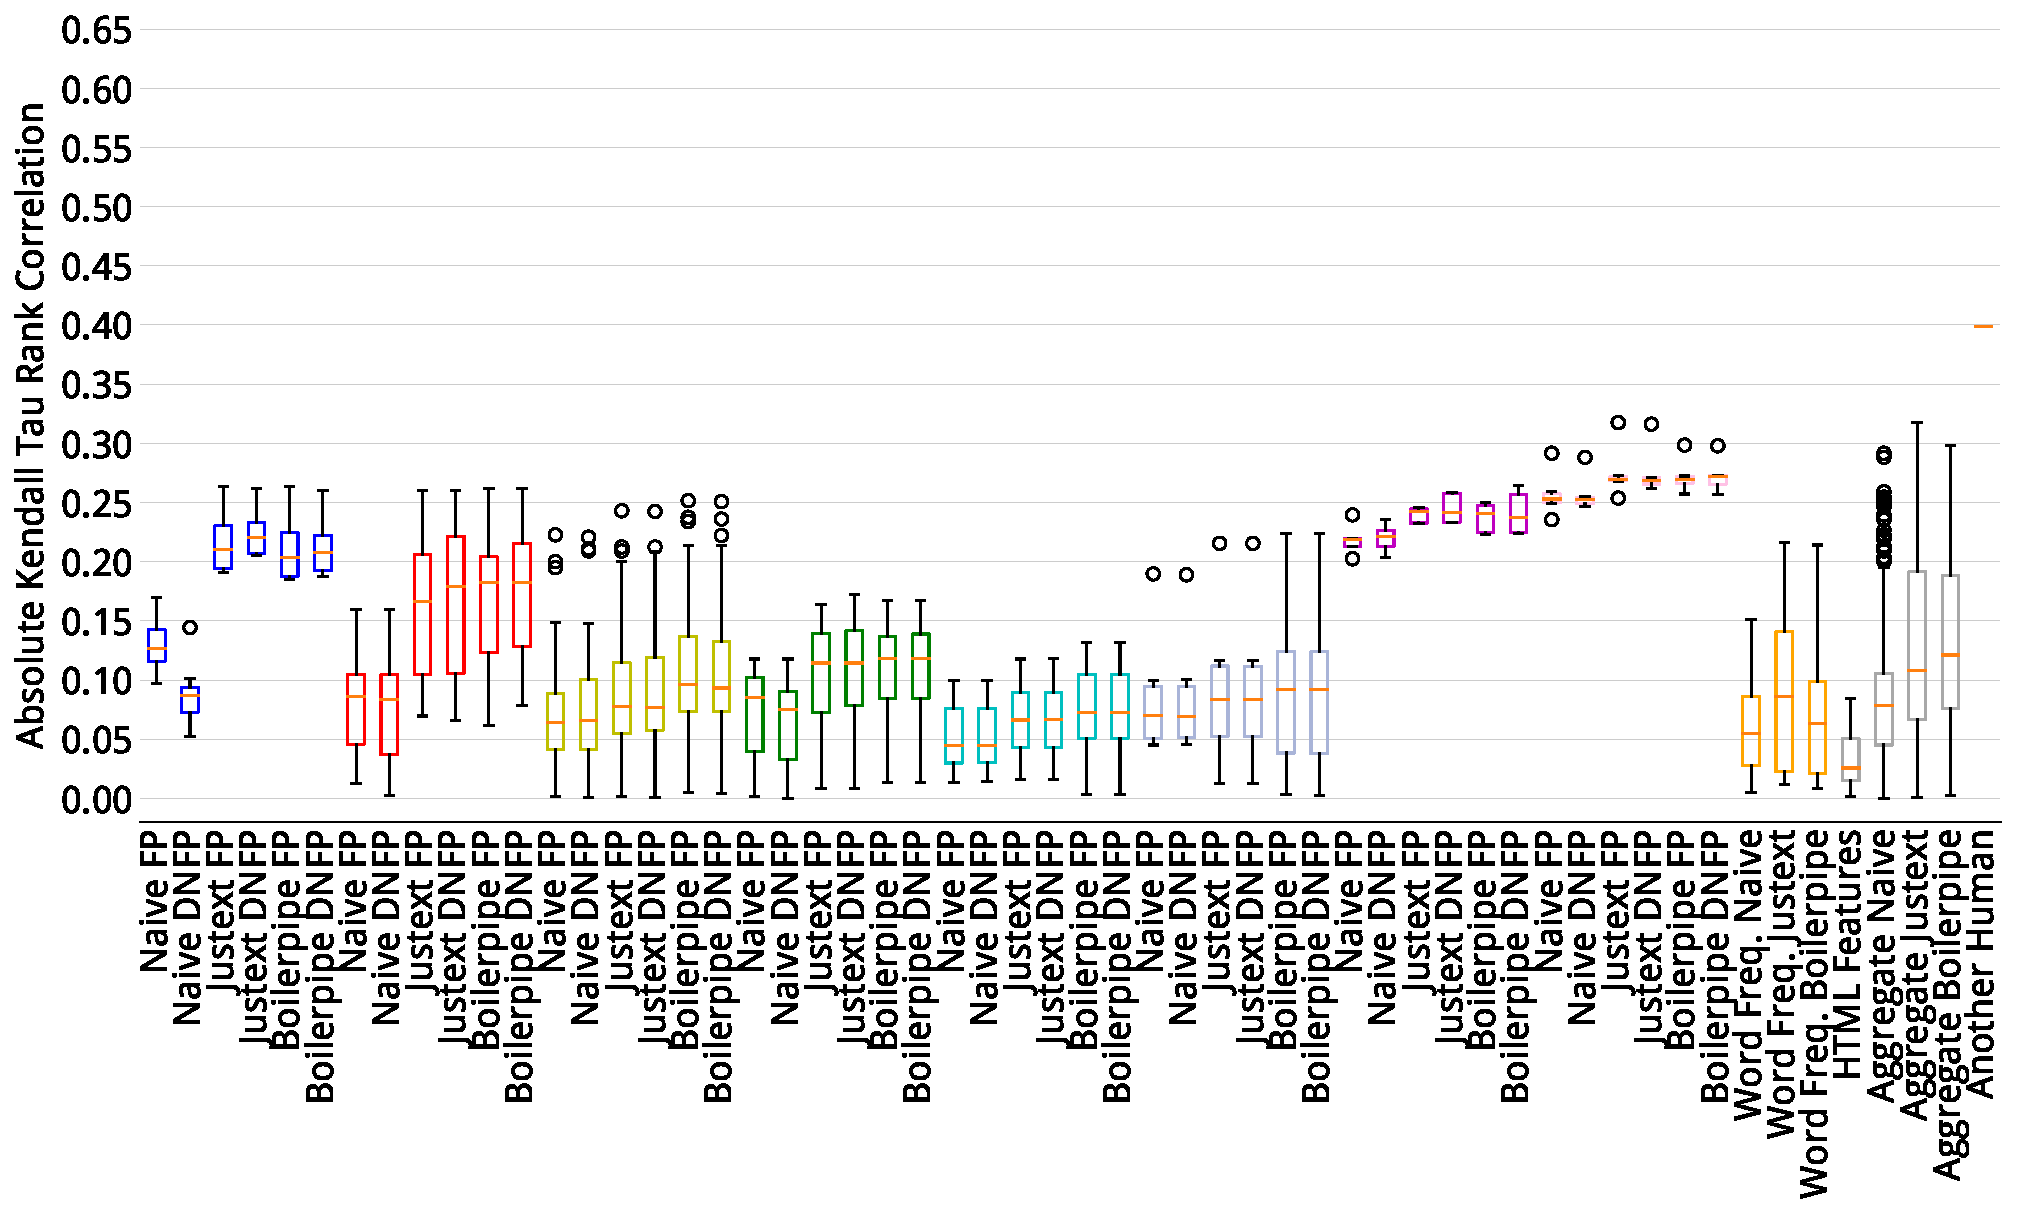
\includegraphics[width=0.90\textwidth]{graphics/box_kendalltau16_raw_values}
%    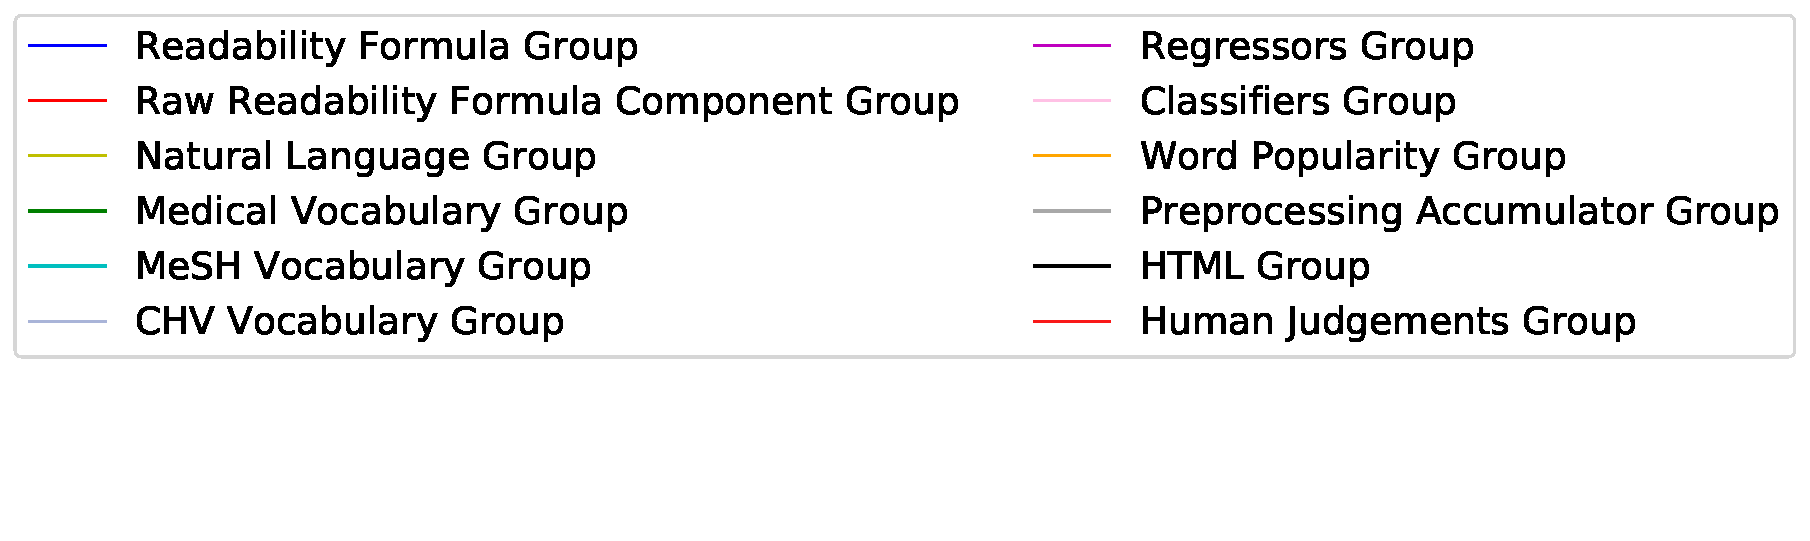
\includegraphics[width=0.65\textwidth]{graphics/legendCorr}
%    \caption{Box plots divided by feature groups. Correlations are calculated using understandability labels from relevant documents assessed in CLEF eHealth 2016}
%   \label{fig:boxplot_corr_docs_2016}
%\end{figure*}

%Figure~\ref{fig:boxplot_corr_docs_2015} shows the correlations for CLEF eHealth 2015 assessments.
%Top part of Figure~\ref{fig:boxplot_corr_docs} shows the Spearman correlation for CLEF eHealth 2015 assessments.

%The choice of preprocessing method had the highest impact on the traditional readability formula group, with the Naive preprocessing clearly underperforming the other preprocessing methods. The choice of the Naive method was also the worst for the word frequency group, but, interestingly, it was a good choice, or at least a competitive one, for all other groups.
%The highest correlations were archived by the regressors and classifiers, independently of the preprocessing method used.

%For this group, all correlation measures point out that the Naive processing yielded the weakest correlation, and Justext was marginally better than Boilerpipe. Comparing the medians, the strategy of DoNotForcePeriod performed better than ForcePeriod. The readability formula group was also the one with higher correlation, with an average correlation equal or higher than the human one.

%Similarly to Figure~\ref{fig:boxplot_corr_docs_2015}, Figure~\ref{fig:boxplot_corr_docs_2016} reports the findings for CLEF eHealth 2016. 
%Similarly the bottom part of Figure~\ref{fig:boxplot_corr_docs} reports the findings for CLEF eHealth 2016. 
%This time, though, the Naive preprocessing method was clearly underperforming for most of the groups analysed, including regressors and classifiers.

%In order to further understand our experiments, we compared the median of each pair of preprocessing strategy showed in Figures~\ref{fig:boxplot_corr_docs_2015} and~\ref{fig:boxplot_corr_docs_2016} and present the results in Table~\ref{tab:comparison_preprocessing}. 

We further analysed the results by performing pairwise comparisons between the median correlations across preprocessing pipelines and heuristics, and reporting the number of times the median correlation of a setting was better than another. These are reported in Table~\ref{tab:comparison_preprocessing}: in brackets we reported the number of comparisons that were statistically significant. 

%In order to further understand our experiments, we present in Table~\ref{tab:comparison_preprocessing} the results of comparing the median of two-by-two for different preprocessing strategies shown in Figure~\ref{fig:boxplot_corr_docs}. We also include the results for Pearson and Kendall correlations.
%For instance, the entry $\mathit{FP < DNFP}$ counts the number of times the median value for \textit{ForcePeriod} was superior to \textit{DoNotForcePeriod} when comparisons with the same HTML cleaning method was used, e.g. \textit{Naive ForcePeriod} versus \textit{Naive DoNotForcePeriod}. From all comparisons, the ones that were statistically significant according to a t-test are shown inside parentheses.

We first examined the comparison between sentence ending heuristics (ForcePeriod (FP) and DoNotForcePeriod (DNFP)). Results showed that the two methods achieved comparable results. Then we examined the comparison between preprocessing pipelines. For these, results for CLEF 2015 were in contrast with those for CLEF 2016. While Naive was marginally better than Boilerpipe and Justext in 2015, it was the worst in the majority of comparisons for 2016. In turn, while Justext was significantly better than Boilerpipe in 2015, they showed balanced results in 2016.
\todo{I think something could be said about ustext and Boilerpipe. Done.}
 

\todo{ARRIVED HERE -- need to merge section 4 and 7.}


%The upper part of Table~\ref{tab:comparison_preprocessing} shows results for the comparisons between ForcePeriod (FP) and DoNotForcePeriod (DNFP). Although the interpretation of readability formulas is drastically affected by this choice of preprocessing, as research indicates~\cite{palotti15}, the correlation results are not.
%The number of times FP reached a higher correlation than DNFP is roughly the same that DNFP was higher than FP.
%The bottom part of Table~\ref{tab:comparison_preprocessing} shows the comparisons made for Naive, Justext and Boilerpipe. Results for CLEF 2015 contrast with 2016, while Naive was sightly better than Boilerpipe and Justext in 2015, it was the worst in almost all 2016 comparisons. Also, the comparisons between Justext and Boilerpipe are exactly the opposite from 2015 to 2016.

%
\begin{table}
\centering    
\caption{Exhaustive Comparison summary using the data from Figures 1.2 and 1.3. Numbers inside parentheses represent the number of tests that yielded p < 0.05 in a two-tailed t-test}
\label{tab:comparison_preprocessing}

\resizebox{1.\textwidth}{!}{
\begin{tabular}{lllllllll}
\toprule
\multirow{2}{*}{\textbf{Comparison}} & \multicolumn{4}{c}{\textbf{CLEF 2015}} & \multicolumn{4}{c}{\textbf{CLEF 2016}}\tabularnewline
\cmidrule(l{2pt}r{2pt}){2-5} \cmidrule(l{2pt}r{2pt}){6-9} 
& \textbf{Pearson} & \textbf{Spearman} & \textbf{Kendall Tau} & \textbf{Total} & \textbf{Pearson} & \textbf{Spearman} & \textbf{Kendall Tau} & \textbf{Total}\tabularnewline
\midrule
FP > DNFP & 8 (0) & 11 (4) & 11 (3) & 30 (7) & 16 (10) & 10 (3) & 11 (4) & 37 (17)\tabularnewline
FP < DNFP & 16 (5) & 12 (5) & 12 (6) & 40 (16) & 8 (0) & 12 (2) & 11 (2) & 31 (4)\tabularnewline
FP == DNFP & 0 & 1 & 1 & 2 & 0 & 2 & 2 & 4\tabularnewline
\midrule
Naive > Justext & 11 (7) & 9 (6) & 9 (5) & 29 (18) & 1 (0) & 0 (0) & 0 (0) & 1 (0)\tabularnewline
Naive < Justext & 6 (4) & 8 (4) & 8 (4) & 22 (12) & 16 (12) & 17 (13) & 17 (13) & 50 (38)\tabularnewline
Naive == Justext & 0 & 0 & 0 & 0 & 0 & 0 & 0 & 0\tabularnewline
Naive > Boilerpipe & 12 (7) & 10 (6) & 10 (5) & 32 (18) & 0 (0) & 0 (0) & 0 (0) & 0 (0)\tabularnewline
Naive < Boilerpipe & 5 (4) & 7 (3) & 7 (3) & 19 (10) & 16 (12) & 17 (13) & 17 (13) & 51 (39)\tabularnewline
Naive == Boilerpipe & 0 & 0 & 0 & 0 & 0 & 0 & 0 & 0\tabularnewline
Justext > Boilerpipe & 10 (7) & 16 (9) & 14 (8) & 40 (24) & 9 (4) & 9 (4) & 4 (2) & 17 (8)\tabularnewline
Justext < Boilerpipe & 7 (2) & 1 (0) & 3 (1) & 11 (3) & 8 (2) & 8 (2) & 13 (2) & 34 (6)\tabularnewline
Boilerpipe == Justext & 0 & 0 & 0 & 0 & 0 & 0 & 0 & 0\tabularnewline
\bottomrule 
\end{tabular}
} % close resizebox
\end{table}

%



%\section{Integrating Understandability into Retrieval}
\label{sec:experiments}

Next, we investigate how understandability estimations could be used and integrated into retrieval methods to increase the quality of search result. To this aim, we first investigated re-ranking search results from an initial run purely based on understandability estimations. 

Specifically, we considered three retrieval methods of differing quality for the initial retrieval. These included the best two runs submitted to each CLEF task (2015 and 2016), and a plain BM25 baseline (default Terrier parameters: $b=0.75$ and $k1=1.2$). As understandability estimators we used  eXtreme Gradient Boosting (XGB)\footnote{For assessed documents, we used 10-fold cross validation, so that we trained XGB on 90\% of the data, and used its predictions for the remaining 10\%. For unassessed documents, we trained XGB on all assessed data, and applied this model to generate predictions.} regressor, as well as SMOG for CLEF 2015 and Dale-Chall for CLEF 2016. These were the best performing approaches from Section~\ref{sec:beyond_readability}.

If all the search results from a run were considered, then such a re-ranking method may place at early ranks Web pages highly likely to be understandable, but possibly less likely to be topically relevant. To balance relevance and understandability, we only re-ranked the first $k$ documents. We explored $k = 15, 20, 50$. Because evaluation was performed with respect to the first $n=10$ rank positions, the setting $k=15$ provided a conservative re-ranking of search results; while, $k=50$ provided a more speculative re-ranking approach. Results are presented in Section~\ref{results:reranking}.

As an alternative to the previous two-step ranking strategy for combining topical relevance and understandability, we explored the fusion of two search results lists separately obtained for relevance and understandability. For this, we used the Reciprocal Rank Fusion (RRF) method~\cite{cormack09}, which has proven effective for combining two lists of search results based on their documents \textit{ranks}, rather than scores. This approach was selected above score-based fusion methods because of the different scoring strategies and distributions employed when scoring for relevance compared to for understandability. For topical relevance, we used, separately, the three methods used for re-ranking (\todo{XXXbest runsXXX} for CLEF2015, GUIR and ECNU for CLEF 2016, and BM25 for both collections). For understandability, we used, separately, the estimations from SMOG/Dale Chall and XGB. Also for this approach we studied limiting the ranking of results to be considered by the methods across the cut-offs $k=15, 20, 50$. Results are presented in Section~\ref{results:fusion}.

Finally, we considered a third alternative to combine topical relevance and understandability: using learning to rank with features derived from the retrieval method and the understandability estimators.
In this experiment, we explored different label attribution and feature sets, keeping the same learning to rank algorithm, again XGB. We first experiment with settings made to optimise only relevance (we consider different Information Retrieval models (BM25, L as feature

\todo{need more details: In the LTR we need to mention the combination of labels to make up the final document label which will be used by the method. Also, we need to say which method we used (pairwise tree boosting) and which are the features for each run.... Note, we only performed learning to rank on the BM25 baseline, because we do not have access to the retrieval features used in the CLEF submissions.}. Results are presented in Section~\ref{results:ltr}.

\begin{table*}[ht!]
\caption{Results obtained by integrating understandability estimations within
retrieval methods on CLEF 2016. Baseline runs are reported at table
indices 1-3. Re-ranking experiments are reported at indices 4-21.
Fusion experiments are reported at indices 22-30. Learning to rank
experiments are reported at indices 31-35. All measures were calculated
up to rank $n=10$. }
%\vspace{-0.2cm}
 \label{tab:experiments} 
\resizebox{1.00\textwidth}{!}{ %
\begin{tabular}{cclllllllllllll}
\toprule 
    \multirow{2}{*}{Index }  & \multirow{2}{*}{Rerank }  & \multirow{2}{*}{Run }  & \multicolumn{4}{l}{Official CLEF 2016 Metrics} & \multicolumn{8}{l}{New Metrics to Evaluate Underst. in Retrieval - Sec.~\ref{sec:data}}\tabularnewline
\cmidrule(l{2pt}r{2pt}){4-7} \cmidrule(l{2pt}r{2pt}){8-15}  &  &  & $RBP$  & RBP Res.  & uRBP  & uRBP Res.  & $RBP_{u}$  & $RBP_{u}$ Res. & $HRBP$  & HRBP Res. & Unj  & $RBP_{r}^{*}$  & $RBP_{u}^{*}$  & $HRBP^{*}$\tabularnewline
\midrule 
1  & \multirow{3}{*}{No Rerank}  & GUIR~\cite{soldaini16} (Best Run)  & \textbf{28.11}  & 7.65  & \textbf{18.12}  & 7.19  & \textbf{45.69}  & 8.86 & \textbf{25.61}  & 6.50 & 0.01  & \textbf{28.29}  & \textbf{46.03}  & \textbf{25.79} \tabularnewline
2  &  & ECNU~\cite{song16} (Runner Up)  & 27.70  & 7.37  & 17.55  & \textbf{7.34}  & 43.89$^{\diamond}$  & 8.66 & 25.35  & 6.26 & 0.01  & 27.77  & 44.18$^{\diamond}$  & 25.48 \tabularnewline
3  &  & Plain BM25 Baseline  & 25.28$^{\diamond}$  & \textbf{8.24}  & 16.05$^{\diamond}$  & 6.94  & 42.08$^{\diamond}$  & \textbf{10.97} & 22.97$^{\diamond}$  & \textbf{7.19} & \textbf{0.06}  & {26.01}$^{\diamond}$  & {43.89}$^{\diamond}$  & {23.93}$^{\diamond}$ \tabularnewline
\midrule 
4  & \multirow{3}{*}{\makecell{Dale-Chall Top 15}}  & Based on GUIR  & 24.70$^{\dagger\diamond}$  & 8.70  & 16.83$^{\dagger\diamond}$  & 7.27  & 49.10$^{\dagger\diamond}$  & 10.62 & 24.94  & 7.50 & 0.03  & 25.24$^{\dagger\diamond}$  & 50.33$^{\dagger\diamond}$  & 25.54 \tabularnewline
5  &  & Based on ECNU  & 24.78$^{\dagger\diamond}$  & 7.83  & 16.64$^{\diamond}$  & 7.16  & 48.88$^{\dagger\diamond}$  & 9.71 & 24.80  & 6.50 & 0.02  & 25.12$^{\dagger\diamond}$  & 49.64$^{\dagger\diamond}$  & 25.21 \tabularnewline
6  &  & Based on BM25  & 23.22$^{\dagger\diamond}$  & 8.78  & 15.85 $^{\diamond}$  & 6.94  & 47.09$^{\dagger\diamond}$  & 11.83 & 24.01  & 7.42 & 0.07  & 24.04$^{\dagger\diamond}$  & 48.60$^{\dagger\diamond}$  & 24.82 \tabularnewline
\hdashline 7  & \multirow{3}{*}{\makecell{Dale-Chall Top 20}}  & Based on GUIR  & 22.19$^{\dagger\diamond}$  & 9.37  & 15.36$^{\dagger\diamond}$  & 6.98  & 48.71$^{\dagger\diamond}$  & 12.30 & 23.21$^{\dagger\diamond}$  & 8.12 & 0.06  & 23.26$^{\dagger\diamond}$  & 51.39$^{\dagger\diamond}$  & 24.45$^{\dagger\diamond}$\tabularnewline
8  &  & Based on ECNU  & 23.01$^{\dagger\diamond}$  & 8.93  & 15.70$^{\dagger\diamond}$  & 6.91  & 48.99$^{\dagger\diamond}$  & 11.69 & 23.73$^{\dagger\diamond}$  & 7.80 & 0.05  & 23.84$^{\dagger\diamond}$  & 51.00$^{\dagger\diamond}$  & 24.66\tabularnewline
9  &  & Based on BM25  & 21.58$^{\dagger\diamond}$  & 9.51  & 14.83$^{\dagger\diamond}$  & 7.02  & 46.99$^{\dagger}$  & 13.00 & 22.89$^{\diamond}$  & 8.06 & 0.09  & 22.93$^{\dagger\diamond}$  & 49.55$^{\dagger\diamond}$  & 24.26\tabularnewline
\hdashline 10  & \multirow{3}{*}{\makecell{Dale-Chall Top 50}}  & Based on GUIR  & 16.18$^{\dagger\diamond}$  & 15.24  & 11.56$^{\dagger\diamond}$  & 6.80  & 41.79$^{\dagger\diamond}$  & 24.49 & 18.10$^{\dagger\diamond}$  & 14.42 & 0.22  & 20.90$^{\dagger\diamond}$  & 53.28$^{\dagger\diamond}$  & 23.27$^{\dagger\diamond}$ \tabularnewline
11  &  & Based on ECNU  & 16.88$^{\dagger\diamond}$  & 17.37  & 11.78$^{\dagger\diamond}$  & \textbf{7.30}  & 40.76$^{\dagger\diamond}$  & 23.77 & 18.30$^{\dagger\diamond}$  & \textbf{15.57} & \textbf{0.24}  & 21.34$^{\dagger\diamond}$  & 52.07$^{\dagger\diamond}$  & 23.33$^{\dagger\diamond}$ \tabularnewline
12  &  & Based on BM25  & 15.06$^{\dagger\diamond}$  & 15.35$^{\dagger\diamond}$  & 10.55  & 6.62  & 40.03 $^{\diamond}$  & 23.88 & 16.55$^{\dagger\diamond}$  & 13.83 & \textbf{0.24}  & 19.42$^{\dagger\diamond}$  & 51.69$^{\dagger\diamond}$  & 21.59$^{\dagger\diamond}$ \tabularnewline
\hdashline 13  & \multirow{3}{*}{\makecell{XGB Top 15}}  & Based on GUIR  & \textbf{25.16}$^{\dagger\diamond}$  & 8.09  & \textbf{17.27}$^{\dagger\diamond}$  & 7.12  & \textbf{50.96}$^{\dagger\diamond}$  & 10.11 & \textbf{25.16}  & 6.89 & 0.02  & \textbf{25.61}$^{\dagger\diamond}$  & 52.00$^{\dagger\diamond}$  & \textbf{25.68}\tabularnewline
14  &  & Based on ECNU  & 24.18$^{\dagger\diamond}$  & 7.69  & 16.54 $^{\diamond}$  & 7.09  & 50.00$^{\dagger\diamond}$  & 9.91 & 24.56  & 6.65 & 0.02  & 24.56$^{\dagger\diamond}$  & 50.74$^{\dagger\diamond}$  & 25.01\tabularnewline
15  &  & Based on BM25  & 22.33$^{\dagger\diamond}$  & 8.14  & 15.46  & 6.76  & 47.90$^{\dagger\diamond}$  & 12.13 & 22.89$^{\diamond}$  & 7.25 & 0.07  & 23.11$^{\dagger\diamond}$  & 49.43$^{\dagger\diamond}$  & 23.69$^{\diamond}$\tabularnewline
\hdashline 16  & \multirow{3}{*}{\makecell{XGB Top 20}}  & Based on GUIR  & 22.38$^{\dagger\diamond}$  & 9.49  & 15.61$^{\dagger\diamond}$  & 7.05  & 50.45$^{\dagger\diamond}$  & 12.08 & 23.30$^{\dagger\diamond}$  & 8.16 & 0.05  & 23.62$^{\dagger\diamond}$  & 52.98$^{\dagger\diamond}$  & 24.68\tabularnewline
17  &  & Based on ECNU  & 22.95$^{\dagger\diamond}$  & 8.82  & 15.95$^{\dagger\diamond}$  & 7.02  & 50.42$^{\dagger\diamond}$  & 11.70 & 23.97$^{\diamond}$  & 7.56 & 0.04  & 23.68$^{\dagger\diamond}$  & 52.15$^{\dagger\diamond}$  & 24.73\tabularnewline
18  &  & Based on BM25  & 20.65$^{\dagger\diamond}$  & 9.42  & 14.46$^{\dagger\diamond}$  & 6.84  & 47.74$^{\dagger\diamond}$  & 13.56 & 21.93$^{\diamond}$  & 8.34 & 0.09  & 21.98$^{\dagger\diamond}$  & 50.28$^{\dagger\diamond}$  & 23.27$^{\diamond}$\tabularnewline
\hdashline 19  & \multirow{3}{*}{\makecell{XGB Top 50}}  & Based on GUIR  & 16.65$^{\dagger\diamond}$  & 15.73  & 12.39$^{\dagger\diamond}$  & 6.84  & 43.49$^{\dagger\diamond}$  & 23.63 & 18.70$^{\dagger\diamond}$  & 13.74 & 0.22  & 21.13$^{\dagger\diamond}$  & \textbf{55.07}$^{\dagger\diamond}$  & 23.58$^{\dagger\diamond}$\tabularnewline
20  &  & Based on ECNU  & 16.19$^{\dagger\diamond}$  & \textbf{17.01}  & 11.82$^{\dagger\diamond}$  & 7.27  & 43.05$^{\diamond}$  & \textbf{24.75} & 18.27$^{\dagger\diamond}$  & 14.41 & \textbf{0.24}  & 20.16$^{\dagger\diamond}$  & 54.70$^{\dagger\diamond}$  & 22.96$^{\dagger\diamond}$\tabularnewline
21  &  & Based on BM25  & 15.43$^{\dagger\diamond}$  & 15.37  & 11.33$^{\dagger\diamond}$  & 6.48  & 41.93$^{\diamond}$  & 23.65 & 17.43$^{\dagger\diamond}$  & 13.40 & 0.26  & 19.58$^{\dagger\diamond}$  & 54.04$^{\dagger\diamond}$  & 22.17$^{\dagger\diamond}$\tabularnewline
\midrule 
22  & \multirow{3}{*}{\makecell{RRF (XGB \& Orig.) Top 15} }  & Based on GUIR  & \textbf{27.23}$^{\dagger\diamond}$  & 7.76  & \textbf{18.31}  & \textbf{7.23}  & 49.69$^{\dagger\diamond}$  & 9.18 & 26.49$^{\dagger\diamond}$  & 6.62 & 0.01  & \textbf{27.46}$^{\dagger\diamond}$  & 50.07$^{\dagger\diamond}$  & \textbf{26.69}$^{\dagger\diamond}$\tabularnewline
23  &  & Based on ECNU  & 26.60$^{\dagger\diamond}$  & 7.41  & 17.81  & 7.19  & 48.67$^{\dagger\diamond}$  & 8.80 & 26.02  & 6.09 & 0.01  & 26.76$^{\dagger\diamond}$  & 49.10$^{\dagger\diamond}$  & 26.27$^{\dagger}$ \tabularnewline
24  &  & Based on BM25  & 24.57$^{\diamond}$  & 8.15  & 16.51$^{\diamond}$  & 6.91  & 46.76$^{\dagger}$  & 11.23 & 24.16$^{\dagger}$  & 7.20 & 0.06  & 25.32$^{\diamond}$  & 48.52$^{\dagger\diamond}$  & 25.08$^{\dagger}$ \tabularnewline
\hdashline 25  & \multirow{3}{*}{\makecell{RRF (XGB \& Orig.) Top 20}}  & Based on GUIR  & 26.21$^{\dagger\diamond}$  & 7.96  & 17.73  & 7.19  & 50.29$^{\dagger\diamond}$  & 9.58 & 25.89  & 6.73 & 0.03  & 26.53$^{\dagger\diamond}$  & 50.98$^{\dagger\diamond}$  & 26.25\tabularnewline
26  &  & Based on ECNU  & 26.15$^{\dagger\diamond}$  & 7.64  & 17.69  & 7.09  & 49.70$^{\dagger\diamond}$  & 9.28 & \textbf{26.07 } & 6.39 & 0.02  & 26.38$^{\dagger\diamond}$  & 50.32$^{\dagger\diamond}$  & 26.35\tabularnewline
27  &  & Based on BM25  & 24.04$^{\dagger\diamond}$  & 8.24  & 16.32$^{\diamond}$  & 6.87  & 47.69$^{\dagger\diamond}$  & 11.40 & 24.08$^{\dagger\diamond}$  & 7.35 & 0.06  & 24.82$^{\dagger\diamond}$  & 49.52$^{\dagger\diamond}$  & 25.01$^{\dagger}$ \tabularnewline
\hdashline 28  & \multirow{3}{*}{\makecell{RRF (XGB \& Orig.) Top 50}}  & Based on GUIR  & 24.09$^{\dagger\diamond}$  & \textbf{9.44}  & 16.85$^{\dagger\diamond}$  & 7.02  & 50.55$^{\dagger\diamond}$  & 11.76 & 24.76  & \textbf{8.01} & 0.07  & 25.08$^{\dagger\diamond}$  & \textbf{52.84}$^{\dagger\diamond}$  & 25.84\tabularnewline
29  &  & Based on ECNU  & 24.17$^{\dagger\diamond}$  & 8.67  & 16.75$^{\diamond}$  & 7.12  & \textbf{50.63}$^{\dagger\diamond}$  & 11.66 & 25.00  & 7.61 & 0.07  & 24.90$^{\dagger\diamond}$  & 52.50$^{\dagger\diamond}$  & 25.84 \tabularnewline
30  &  & Based on BM25  & 22.28$^{\dagger\diamond}$  & 8.87 & 15.50  & 6.76  & 48.79$^{\dagger\diamond}$  & \textbf{12.90} & 23.13$^{\dagger\diamond}$  & 7.82 & \textbf{0.10 } & 23.46$^{\dagger\diamond}$  & 51.89$^{\dagger\diamond}$  & 24.57\tabularnewline
\midrule 
31  & \multirow{5}{*}{XGB LeToR}  & Combo 1 on BM25  & 20.42$^{\dagger\diamond}$  & 17.61  & 13.00$^{\dagger\diamond}$  & 7.41  & 32.17$^{\dagger\diamond}$  & 24.61 & 18.39$^{\dagger\diamond}$  & 14.41 & 0.28  & 25.25$^{\diamond}$  & 43.19$^{\diamond}$  & 23.83$^{\diamond}$\tabularnewline
32  &  & Combo 2 on BM25  & 24.98$^{\dagger\diamond}$  & 19.83  & 15.30$^{\dagger\diamond}$  & 8.09  & 35.09$^{\dagger\diamond}$  & 25.14 & 22.26$^{\diamond}$  & 17.50 & 0.24  & 30.41  & 46.09  & 28.28$^{\dagger\diamond}$ \tabularnewline
33  &  & Combo 3 on BM25  & 26.35$^{\dagger}$  & \textbf{20.48}  & 15.88$^{\dagger\diamond}$  & 8.16  & 34.73$^{\dagger\diamond}$  & 24.69 & 21.81$^{\dagger}$  & 17.41 & 0.22  & 32.25$^{\diamond}$  & 45.44  & 28.22$^{\dagger\diamond}$\tabularnewline
34  &  & Combo 4 on BM25  & 16.16$^{\dagger\diamond}$  & 19.48  & 10.76$^{\dagger\diamond}$  & 7.27  & \textbf{36.75}$^{\dagger\diamond}$  & \textbf{28.51} & 16.77$^{\dagger\diamond}$  & \textbf{17.80} & \textbf{0.29 } & 22.20$^{\dagger\diamond}$  & \textbf{50.06}$^{\dagger\diamond}$  & 23.32$^{\diamond}$\tabularnewline
35  &  & Combo 5 on BM25  & \textbf{26.76}$^{\diamond}$  & \textbf{20.48}  & \textbf{16.19}$^{\diamond}$  & \textbf{8.34}  & 35.26$^{\dagger\diamond}$  & 24.13 & \textbf{22.96}  & 17.59 & 0.22  & \textbf{32.60}$^{\dagger}$  & 45.87  & \textbf{29.20}$^{\dagger\diamond}$\tabularnewline
\bottomrule
\end{tabular}
} % end of resizebox
\end{table*}



\vspace{-10pt}
\section{Evaluation of Understandability Retrieval}
\label{sec:results}

We report the results obtained when experimenting with the retrieval methods described above in Table~\ref{tab:experiments}. We report only the results for CLEF 2016 (thus we only report Dale Chall) for brevity; those on CLEF 2015 exhibited similar trends and are included in the online appendix. The effectiveness of the top two submission to CLEF 2016 and the BM25 baseline are reported at indices 1-3 of the table. Statistical significant differences compared to the best participating run, GUIR, are reported with $\diamond$; differences between the original run (indices 1-3) and its modification are reported with $\dagger$ (paired, two-tail t-test, $p<0.05$). Note that the baseline BM25 is significantly worse than GUIR across all measures. \todo{JP: actually note that the dagger IS NOT a comparison with ECNU, rather it is comparing a modified run with the original version} 

%We start our experiments by showing at the top of Table~\ref{tab:experiments} (indices 1-3) the performance of the top 3 systems in CLEF eHealth 2016 together with a straightforward BM25 baseline run made with Terrier toolkit. Our further experiments will use not only these runs as a comparison base, but modify these runs when necessary.

\subsection{Re-ranking}
\label{results:reranking}

Indices 4-6 of Table~\ref{tab:experiments} report on our experiments re-ranking documents from runs listed at indices 1-3, up to rank 20, according to their Dale-Chall index.
We find that the topical relevance of the re-ranked runs, represented by $NDCG_r$ significantly decreases when compared to their original runs. For example, the $NDCG_r$ of the re-ranked Dale-Chall version of BM25 decreased from 22.02 to 18.53. However, the re-ranked results were significantly more understandable, as reported by their $NDCG_u$. 
Note a limitation of RBP or uRBP metrics to reveal such trend, as both relevance and understandability are tied together.
% As the number of unassessed documents increases ($Una@10$)

Next, we swap the Dale-Chall Index by XGB regressor trained using all features of Table~\ref{tab:doc_features}\footnote{Experiments with various Machine Learning methods and feature selection schemes were performed as well and are available in the online appendix. The results of other methods are similar.}. % When using the set of top 10 features for each group from Table~\ref{tab:top_corr_metrics} results are always better than using an automatic method such as Chi Square to select 10 features to use.}.
%While the higher correlation of Dale-Chall was XXX (as reported in table Y), correlations using XGB reached YYY, the closest method to the human agreement in this task.
We experiment with re-ranking at cut-off 15 (more more conservative method), 20 and 50 (a more heterodox method). 
A similar understandability-relevance trade-off is seen when using a machine learning regressor in place of the Dale-Chall index.
Note that, for the same cut-off value\footnote{We shown here only Dale-Chall cut-off of 20 for brevity.}, the machine learning method consistently yields more understandable results (higher $NDCG_u$). 

\subsection{Rank Fusion}
\label{results:fusion}

Next, from the index 16 to 24, we report the results of our approach to automatically combine topical relevance and understandability through rank fusion.
Once more, allowing re-ranks at higher cut-offs result in larger gains in terms of understandability, but in small losses in terms of topical relevance.
However, the combination of understandability and relevance, $H_ru$, is more stable now than for the previous re-rank methods. 
For example, compare the $H_{ru}^*$ of 13 (21.97) and 22 (24.34) with the original run at index 1 (24.77).

\subsection{Learning to Rank}
\label{results:ltr}

Last, we evaluate our experiments with learning to rank. 


Our final batch of experiments, indices 32-34, are based on learning-to-rank. We decided to use the pairwise implementation of the gradient boosting approach from the XGBoost framework~\cite{chen16} due to its recent good results in many machine learning tasks \todo{actually, I should use XGBoost method instead of LR}. Evaluating other learning to rank methods and frameworks are left as future work.
We evaluated three different settings based on the plain BM25 run shown in index 4, each one with a different combination of feature set and relevance labels:
\begin{itemize}
    \item Index 32: we used as relevance labels only the topical labels and as feature set the score of different information retrieval models (BM25, Dirichlet LM and PL2). This represents the typical use of learning to rank aiming to optimize only the topical relevance results. Unfortunately that was not the case and not even the $P_r@10*$ was improved.
    \item Index 33: we used as relevance labels the linear combination of topical relevance and understandability. Additionally to the IR features, we used the 10 features correspondent to the best features according to Kendall tau in Table~\ref{tab:top_corr_metrics}. Results show that this resulted in higher $F_{ur}*$ when compared to its correspondent approaches (indices 4, 8, 12, 16, 19, 23, 27 and 31) due to a high increase in $P_r@10*$, which reveals understandability features improving topicability.
    \item Index 34: On top of our previous run, we included here all features shown in Table~\ref{tab:doc_features}. Note that despite the very high number of unassessed documents, this run shows improvements even in $P_r@10$ obtaining the same results as the third best run in the campaign (ECNU). In its turn, the $P_{r}*$ which ignores the unassessed documents is 8.4\% higher than the best system, while $F_{ru}*$ is 5.2\% higher.
\end{itemize}






%
\section{Conclusion}
\label{sec:conclusion_doc_analysis}

In this paper we have examined approaches to estimate the understandability of health Web pages, including the impact of HTML preprocessing techniques, and how to integrate these within retrieval methods to provide more understandable search results for people seeking health information. 

The empirical experiments suggested that: (1) machine learning methods based on regression are best suited to estimate the understandability of health Web pages; (2) preprocessing does affect effectiveness (both for understandability prediction and document retrieval), although, compared to other methods, ML-based methods for understandability estimation are less subject to variability due to poor preprocessing; (3) learning to rank methods can be specifically trained to promote more understandable search results. 

This paper makes a clear contribution to improving search engines tailored to consumer health search because it thoroughly investigates promises and pitfalls of understandability estimations and their integration into retrieval methods. The paper further highlights which methods and settings do provide better search results to health information seekers. As shown in Figure~\ref{fig:dist}, these methods would clearly improve current health-focused search engines. 


%\mytodo{Needs to be re-written}
%
%There is an abundance of factors that affect how readability is perceived by users. 
%In this paper we devised and studied a large number of readability estimators, ranging from traditional readability formulas extensively used in the past 50 years to state-of-the-art machine learning algorithms.
%We grouped them into semantically related groups in order to visualize their correlation with human assessments collected during CLEF eHealth campaigns in 2015 and 2016.
%
%Complementary to the literature research~\cite{palotti15}, we evaluated how preprocessing steps impact the readability estimation in traditional readability formulas and in other modern estimators. We empirically learnt the importance of preprocessing steps when applying readability formulas, as the highest correlations happen when other than the Naive method is used.
%For the most modern estimators, such as the ones based on machine learning methods, the correlation is less sensitive to the preprocessing steps.
%
%We also studied the correlation of each individual readability formula with the human assessment to provide insights into which formula should be preferred. Our analysis concluded that the Simple Measure of Gobbledygook (SMOG) and Dale-Chall Index (DCI) were the most correlated metrics for the two datasets studied and, together with Coleman-Liau Index (CLI) and the Flesch Reading Ease (FRE) are the most stable metrics across datasets, and therefore, should be preferred.




%\newpage
\bibliographystyle{ACM-Reference-Format}
\bibliography{main} 

\end{document}
